%\part{Experimantal Implementation}
\chapter{Experimental Verification}
\section{RT-HYTEM of Substructuring technique}
\subsection{Experimental Result and Discussion}
The validity of the proposed real-time substructuring technique is verified for the experimental setting described in the previous sections. First, the shaking table test without feedback loop of accelerations measured from the experimental substructure into the shaking table controller in Figure~\ref{fig:2-11} is performed to experimentally confirm the validity of the proposed method. In this case, the third story acceleration of responses pre-calculated from the assumed whole building with structural parameters such as Eqs.~\eqref{eq:2-18} and \eqref{eq:2-19} is used as a reference signal in Figure~\ref{fig:2-8}. Figure~\ref{fig:2-12} compares the time histories and Fourier transform of the acceleration responses, which are measured from the experimental substructure and shaking table, with those calculated from the numerical analysis of the assumed whole structure. In other words, the responses corresponding to the 3rd, 4th and 5th story accelerations are compared. Also, Figures~\ref{fig:2-13}-\ref{fig:2-15} showing the variation of frequency components according to time lapse illustrate the spectrogram and contour plots of experimental and numerical accelerations of the 3rd, 4th and 5th story, respectively. As can be confirmed from Figure~\ref{fig:2-12}, the experimental accelerations obtained from the shaking table test without their feedback agree well with those obtained from the analysis of the assumed whole structure in both time and frequency domains. However, it can be observed that the small discrepancies are shown in the time histories of 4th and 5th story accelerations as shown from Figure~\ref{fig:2-12}, while the 3rd story acceleration is identical to the numerical one over the entire time history as known from Figures~\ref{fig:2-12}-\ref{fig:2-13}. These differences are caused by the inherent modes of experimental substructure; the frequency components of 2.5 and 8.6 Hz corresponding to the first and second modes of the experimental substructure, respectively, are observed in the measured acceleration of 4th story as known from Figure~\ref{fig:2-14}, and also the component of 2.5 Hz is expressed in the 5th story experimental acceleration as like Figure~\ref{fig:2-15}. It is considered that this tendency is especially conspicuous in case of utilizing a lightly-damped testing model as an experimental substructure. Table 1 shows the frequency components observed in the time records of an experimental substructure from the test without its acceleration feedback and the natural frequencies calculated from the assumed whole structure with five stories. From Table~\ref{tab:2-1}, it can be noted that the first natural frequency of the experimental substructure is shifted from 2.5 Hz to 1.3 Hz by the dynamics of the three-story numerical substructure added to its base.
 Then, the real-time substructuring shaking table test expressed as Figure~\ref{fig:2-11} was carried out based on the acceleration feedback of the experimental substructure. Figure~\ref{fig:2-16} compares the responses measured from the test with the acceleration feedback of the experimental substructure with those calculated from the numerical analysis of the assumed whole structure with 5 DOFs. Also, Figures~\ref{fig:2-17}-\ref{fig:2-19} express the frequency components according to time lapse, which are observed in the measured responses from the test with feedback and the calculated ones of the 3rd, 4th and 5th story, respectively. As known from Figure~\ref{fig:2-16}, the inclination in entire time history responses measured from the proposed testing method agrees well with that calculated from the assumed whole structure. This is why the first mode responses of substructured system coincide well with those of the assumed whole system over the entire time range, as shown in Figures~\ref{fig:2-17}-\ref{fig:2-19}. However, as can be confirmed from Figures~\ref{fig:2-17}-\ref{fig:2-19}, instead of the 2nd and 3rd mode responses of substructured system, those of the experimental substructure are observed from the testing results in the vicinity of 2.5 and 8.6 Hz. It is considered that in the process of the acceleration feedback of the experimental substructure, its fundamental modes affect to the numerical substructure and then numerical error occurs in calculating the numerical substructure.

\begin{figure}[ht]
\centering
\subfigure[Time domain]{
   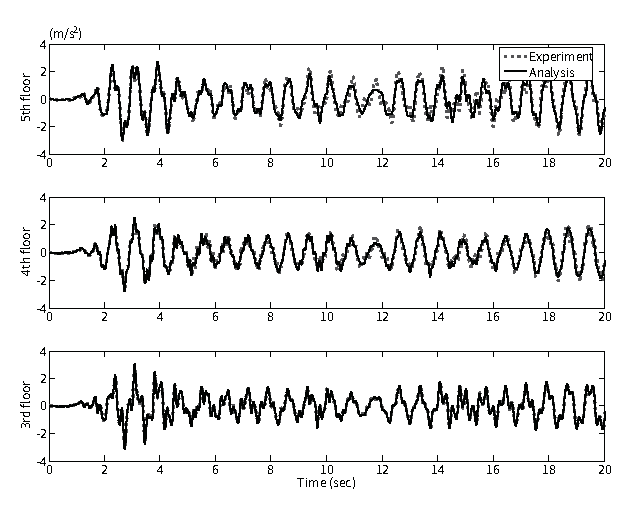
\includegraphics[width=0.8\textwidth] {figure/2-12a.eps}
   \label{fig:2-12a}
 }
 \subfigure[Frequency domain]{
   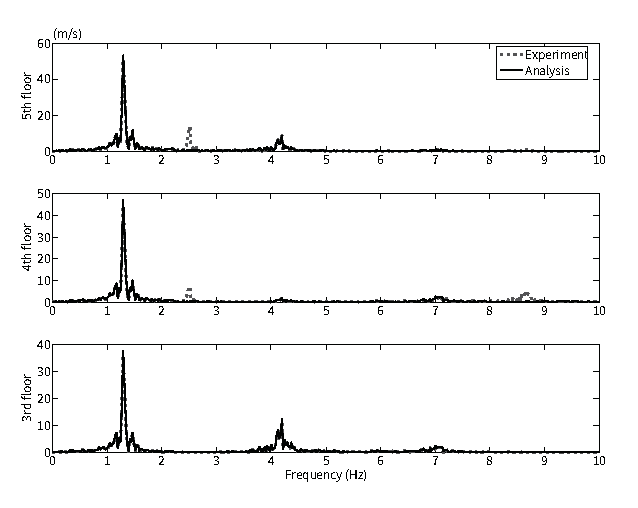
\includegraphics[width=0.8\textwidth] {figure/2-12b.eps}
   \label{fig:2-12b}
 }
\caption{Comparisons of results measured from the experiment without feedback and those calculated from numerical analysis.}
\label{fig:2-12}
\end{figure}

\begin{figure}[ht]
\centering
 \subfigure[Spectrogram of the response measured from the experiment without feedback]{
   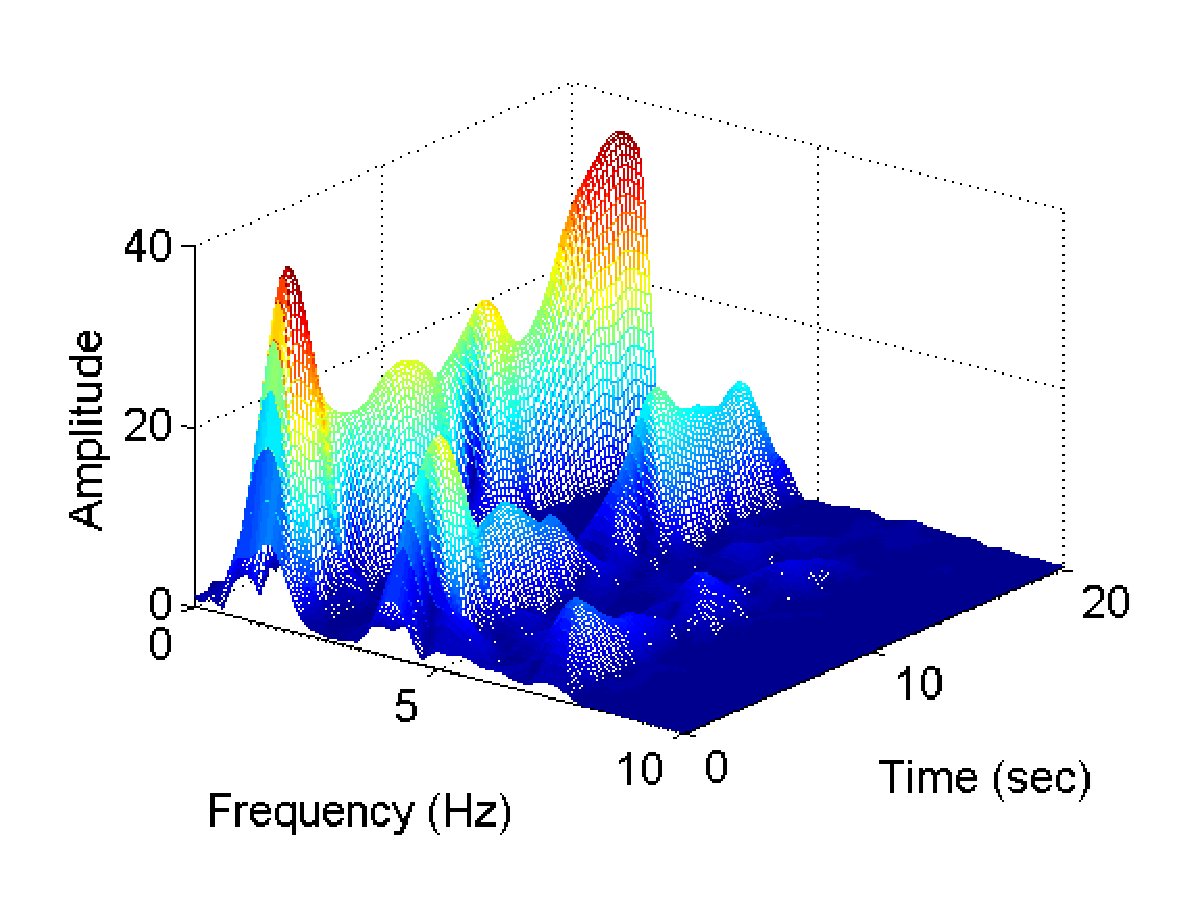
\includegraphics[width=0.45\textwidth] {figure/2-13a.eps}
   \label{fig:2-13a}
 }\hfill
 \subfigure[Spectrogram of the response calculated from the numerical analysis measured]{
   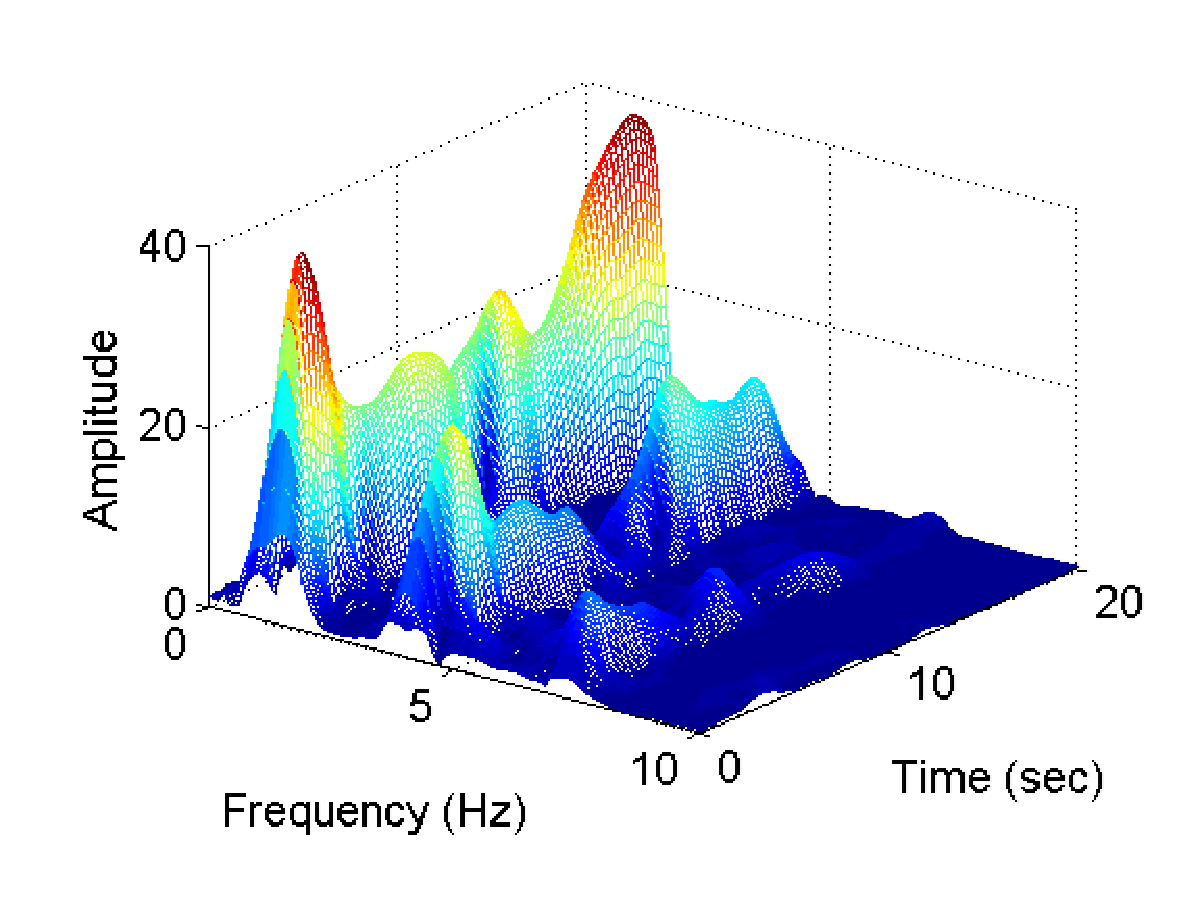
\includegraphics[width=0.45\textwidth] {figure/2-13b.eps}
   \label{fig:2-13b}
 }
 \subfigure[Contour plot of the response measured from the experiment without feedback]{
   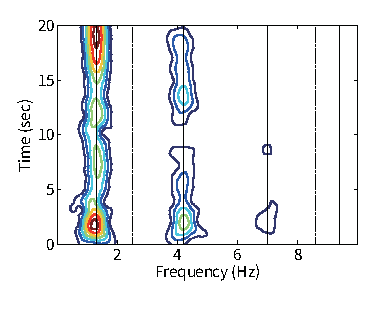
\includegraphics[width=0.45\textwidth] {figure/2-13c.eps}
   \label{fig:2-13c}
 }\hfill
 \subfigure[Contour plot of the response calculated from the numerical analysis measured]{
   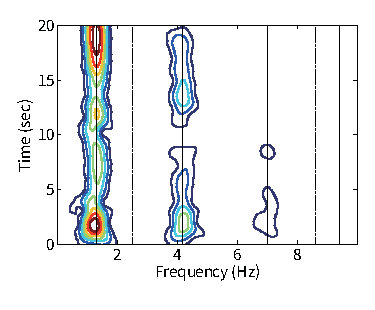
\includegraphics[width=0.45\textwidth] {figure/2-13d.eps}
   \label{fig:2-13d}
 }
\caption{Spectrograms and contour plots of the 3rd story acceleration measured from the experiment without feedback and that calculated from the numerical analysis.}
\label{fig:2-13}
\end{figure}

\begin{figure}[ht]
\centering
 \subfigure[Spectrogram of the response measured from the experiment without feedback]{
   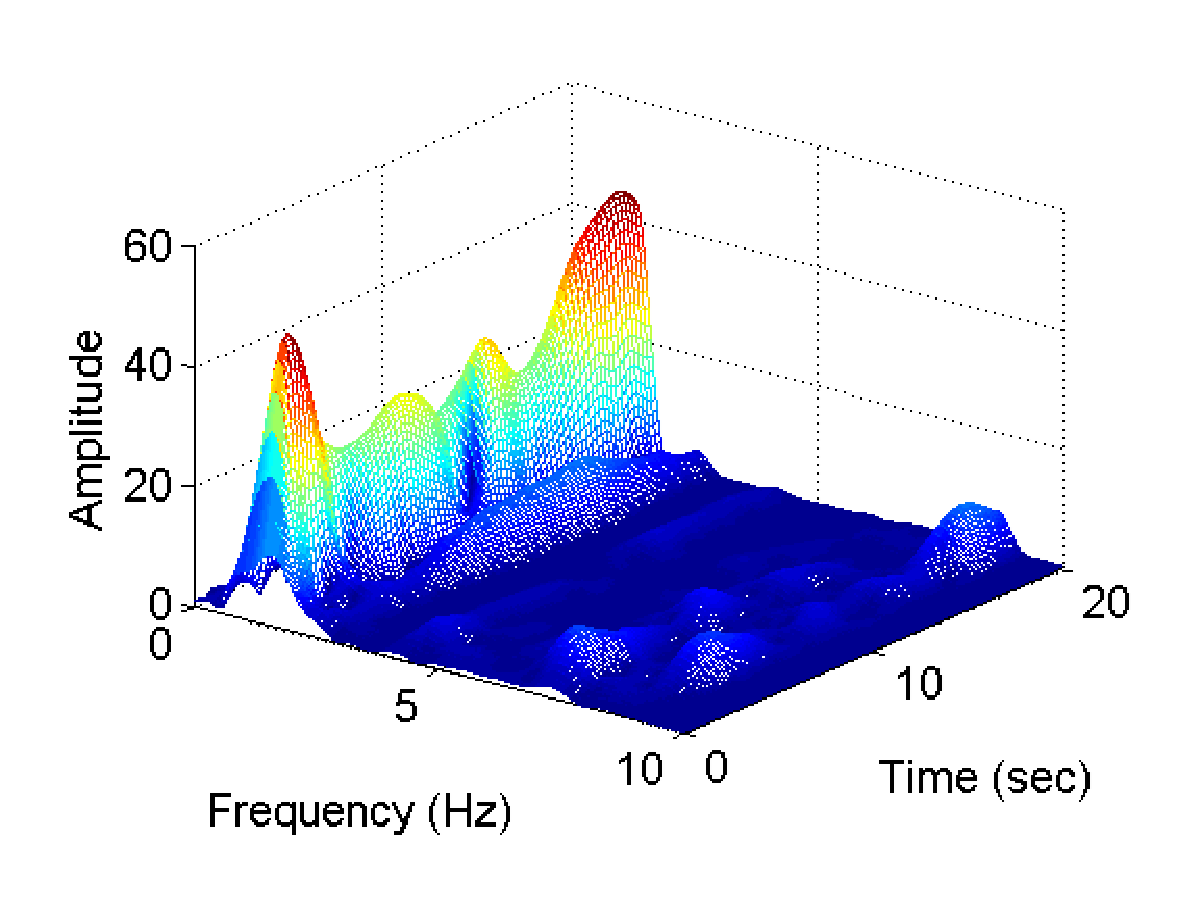
\includegraphics[width=0.45\textwidth] {figure/2-14a.eps}
   \label{fig:2-14a}
 }\hfill
 \subfigure[Spectrogram of the response calculated from the numerical analysis measured]{
   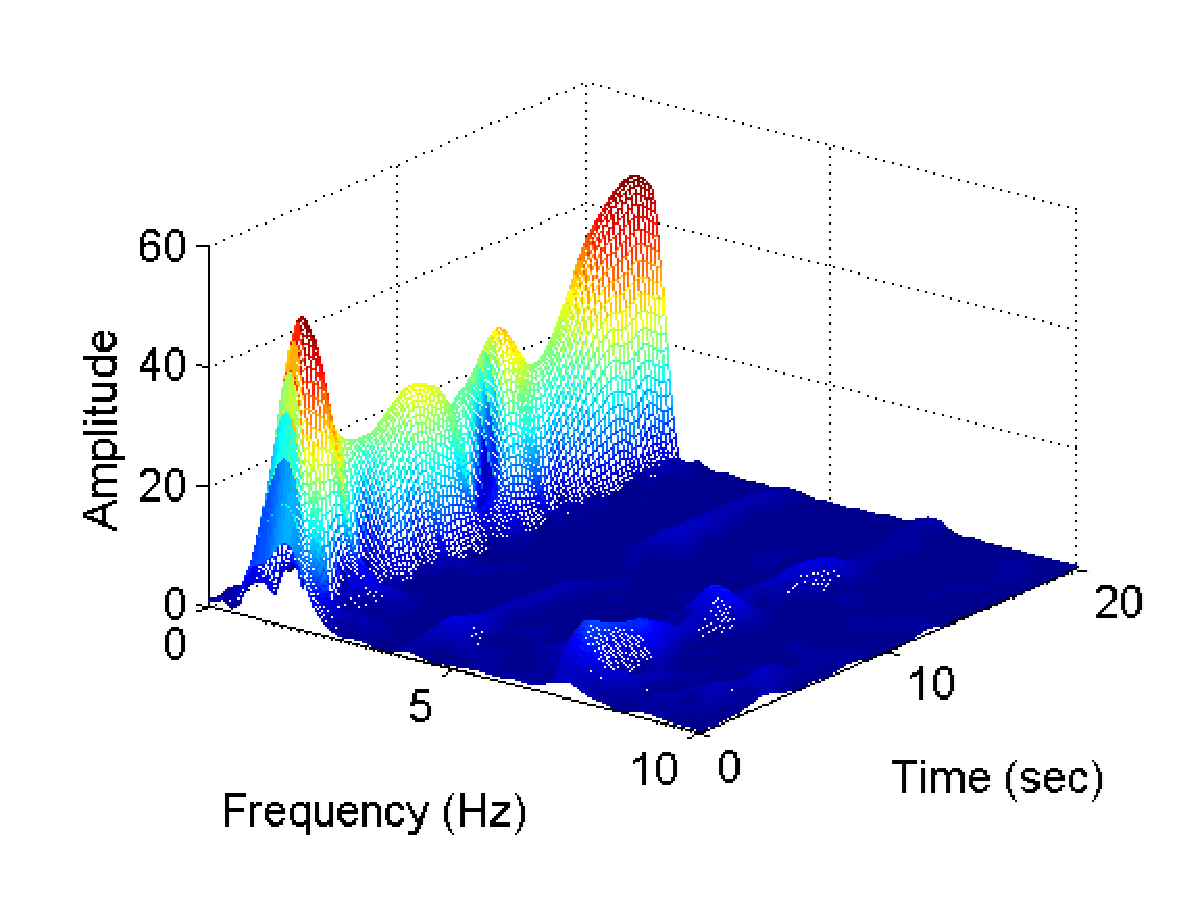
\includegraphics[width=0.45\textwidth] {figure/2-14b.eps}
   \label{fig:2-14b}
 }
 \subfigure[Contour plot of the response measured from the experiment without feedback]{
   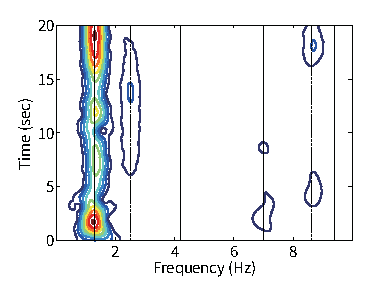
\includegraphics[width=0.45\textwidth] {figure/2-14c.eps}
   \label{fig:2-14c}
 }\hfill
 \subfigure[Contour plot of the response calculated from the numerical analysis measured]{
   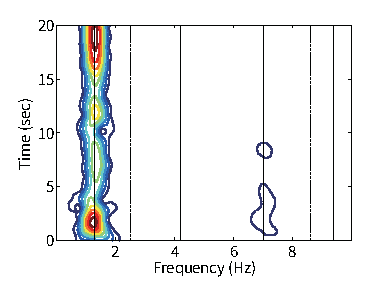
\includegraphics[width=0.45\textwidth] {figure/2-14d.eps}
   \label{fig:2-14d}
 }
\caption{Spectrograms and contour plots of the 4th story acceleration measured from the experiment without feedback and that calculated from the numerical analysis.}
\label{fig:2-14}
\end{figure}

\begin{figure}[ht]
\centering
 \subfigure[Spectrogram of the response measured from the experiment without feedback]{
   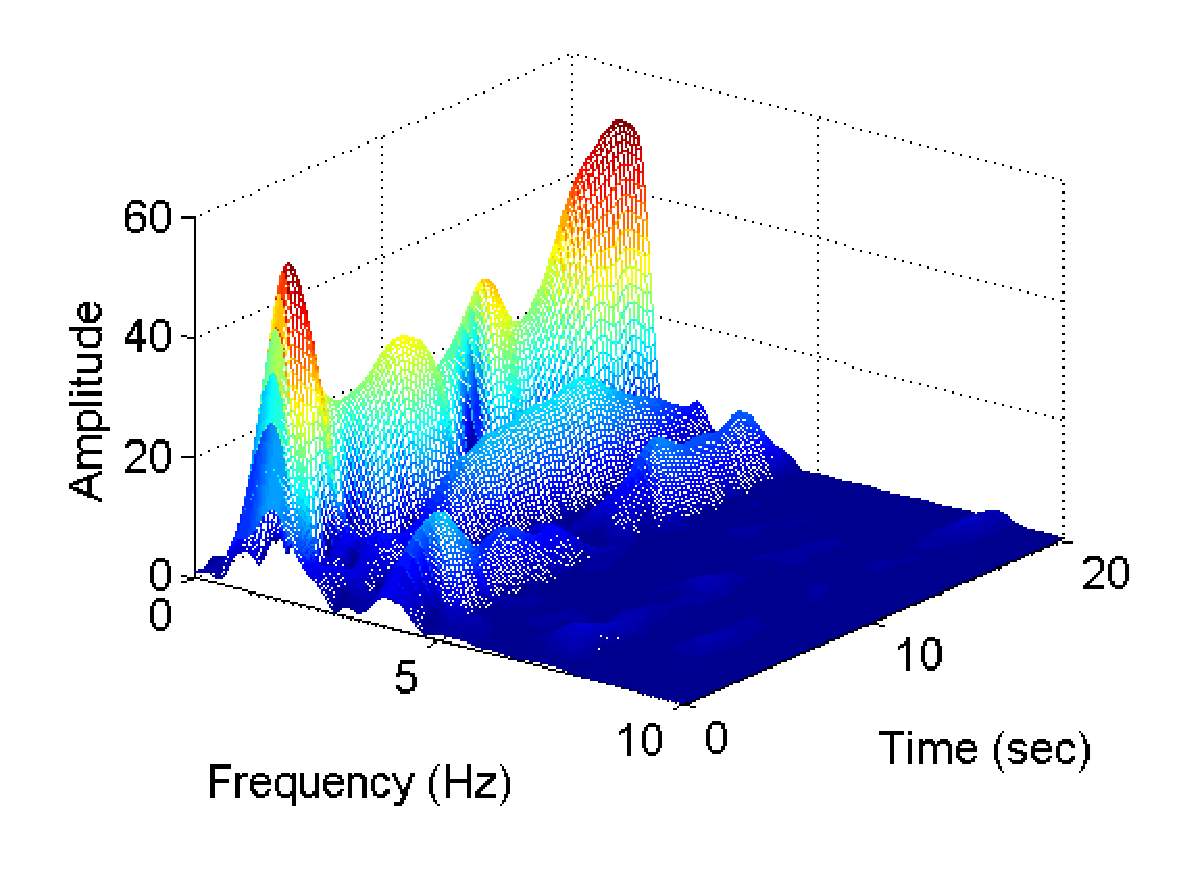
\includegraphics[width=0.45\textwidth] {figure/2-15a.eps}
   \label{fig:2-15a}
 }\hfill
 \subfigure[Spectrogram of the response calculated from the numerical analysis measured]{
   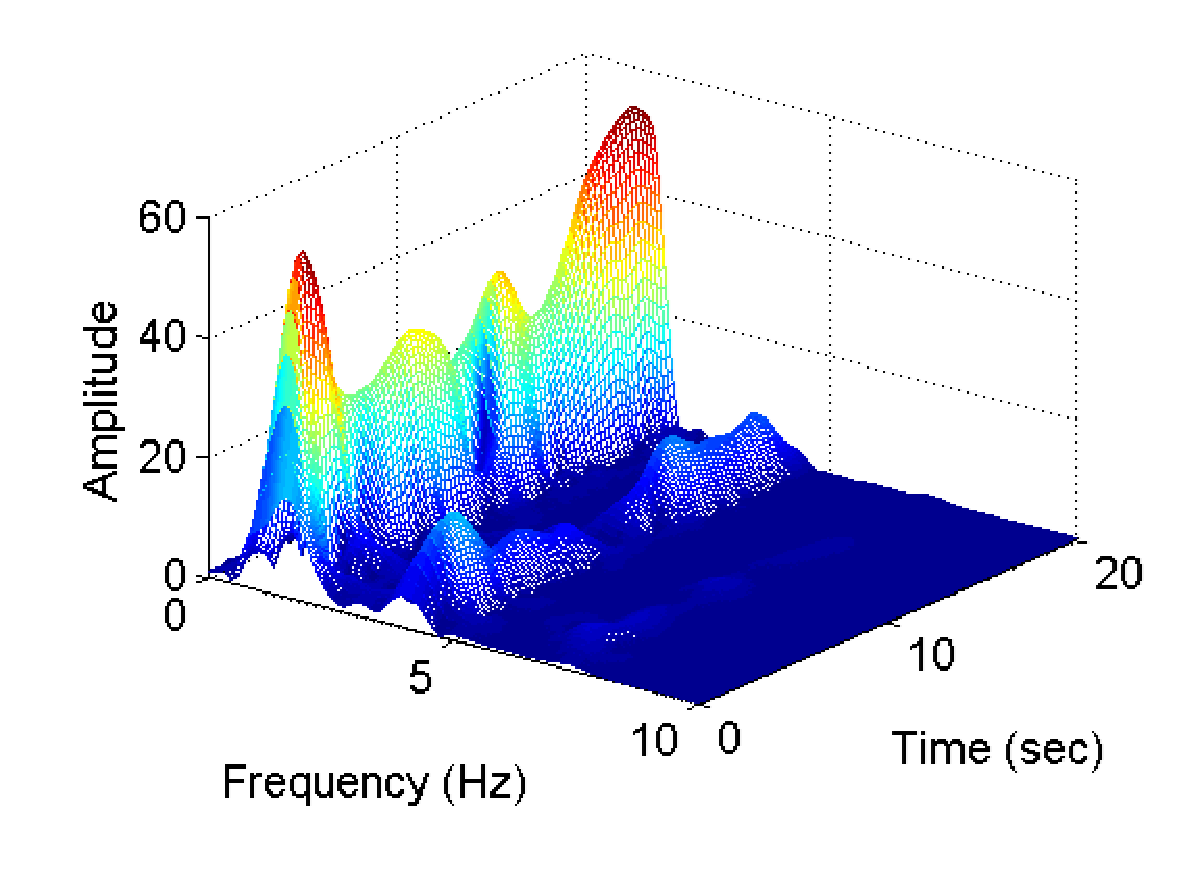
\includegraphics[width=0.45\textwidth] {figure/2-15b.eps}
   \label{fig:2-15b}
 }
 \subfigure[Contour plot of the response measured from the experiment without feedback]{
   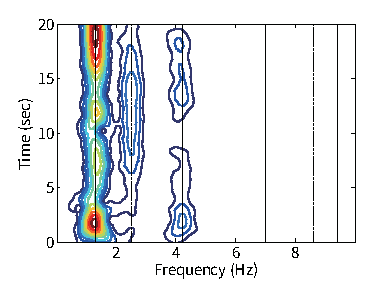
\includegraphics[width=0.45\textwidth] {figure/2-15c.eps}
   \label{fig:2-15c}
 }\hfill
 \subfigure[Contour plot of the response calculated from the numerical analysis measured]{
   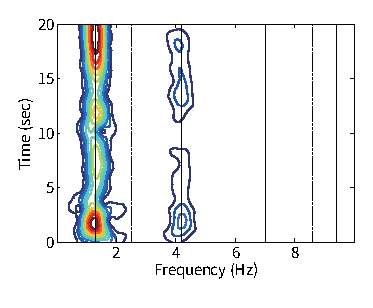
\includegraphics[width=0.45\textwidth] {figure/2-15d.eps}
   \label{fig:2-15d}
 }
\caption{Spectrograms and contour plots of the 5th story acceleration measured from the experiment without feedback and that calculated from the numerical analysis.}
\label{fig:2-15}
\end{figure}

\begin{figure}[ht]
\centering
\subfigure[Time domain]{
   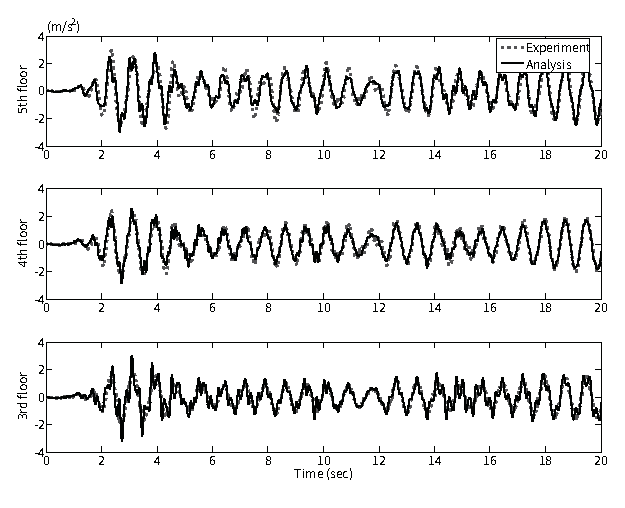
\includegraphics[width=0.8\textwidth] {figure/2-16a.eps}
   \label{fig:2-16a}
 }
 \subfigure[Frequency domain]{
   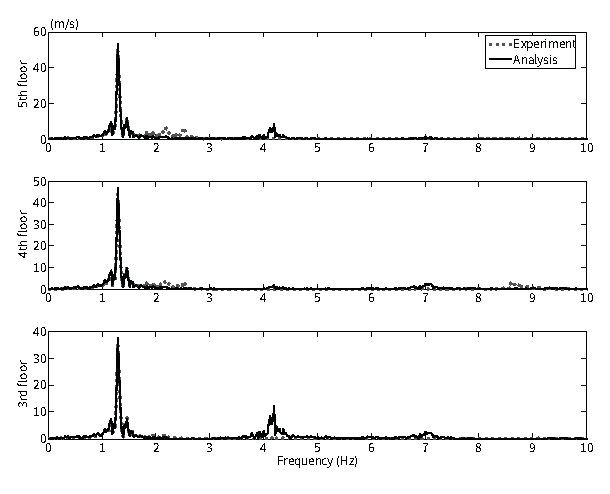
\includegraphics[width=0.8\textwidth] {figure/2-16b.eps}
   \label{fig:2-16b}
 }
\caption{Comparisons between results from the experiment with feedback and those from analysis.}
\label{fig:2-16}
\end{figure}

\begin{figure}[ht]
\centering
 \subfigure[Spectrogram of the response measured from the experiment without feedback]{
   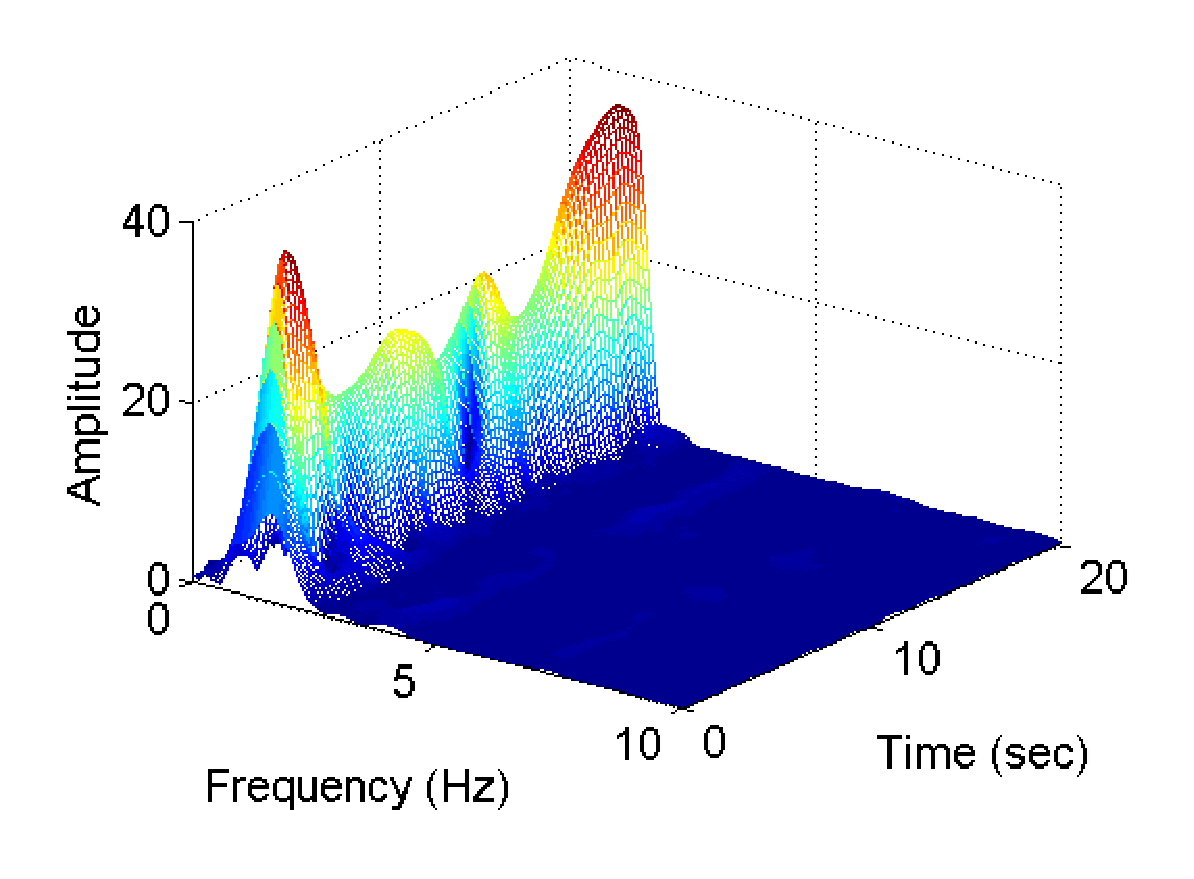
\includegraphics[width=0.45\textwidth] {figure/2-17a.eps}
   \label{fig:2-17a}
 }\hfill
 \subfigure[Spectrogram of the response calculated from the numerical analysis measured]{
   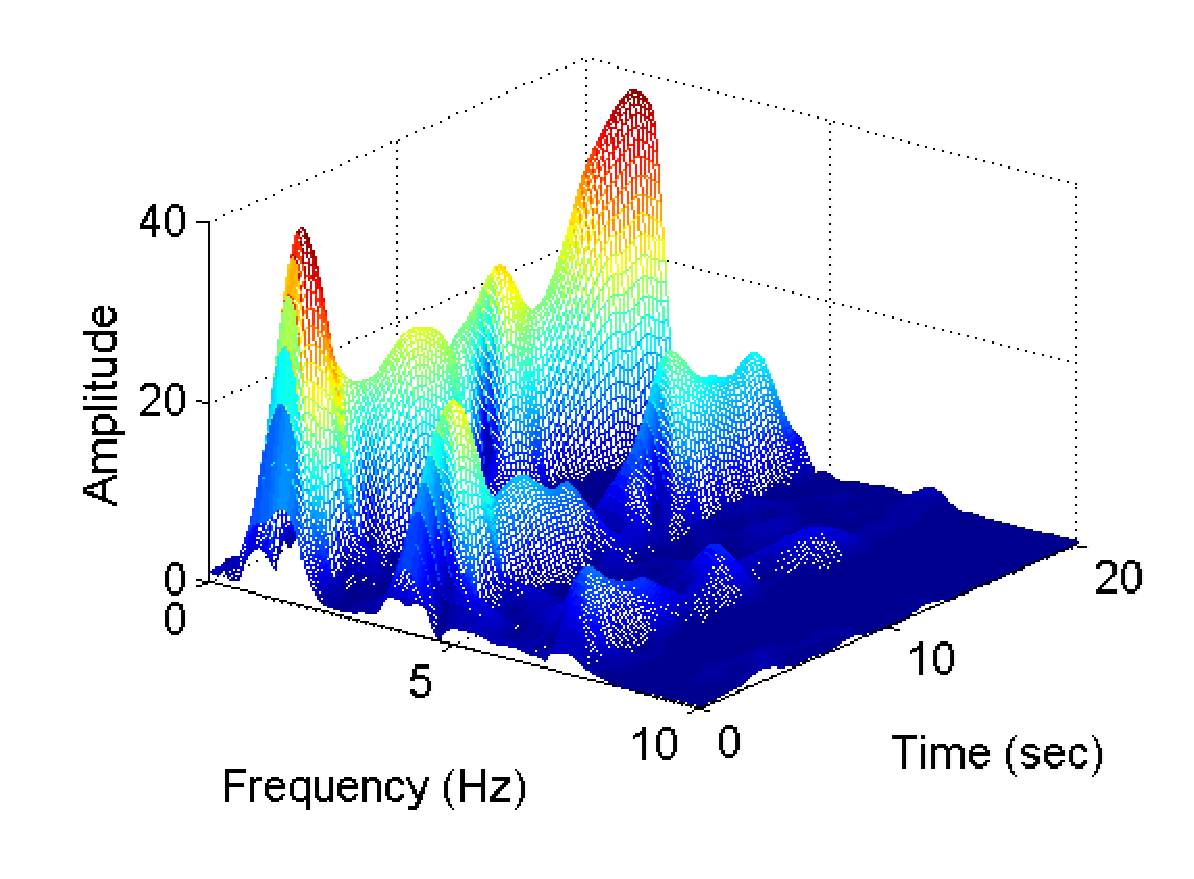
\includegraphics[width=0.45\textwidth] {figure/2-17b.eps}
   \label{fig:2-17b}
 }
 \subfigure[Contour plot of the response measured from the experiment without feedback]{
   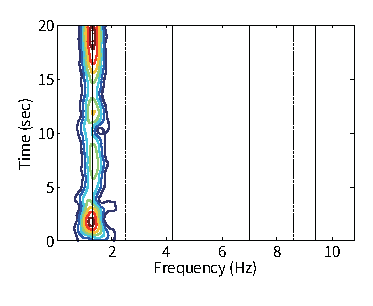
\includegraphics[width=0.45\textwidth] {figure/2-17c.eps}
   \label{fig:2-17c}
 }\hfill
 \subfigure[Contour plot of the response calculated from the numerical analysis measured]{
   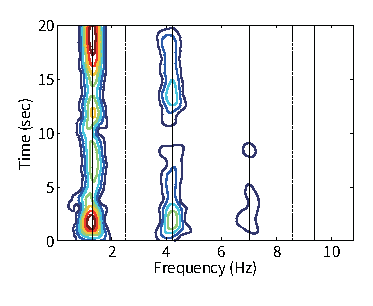
\includegraphics[width=0.45\textwidth] {figure/2-17d.eps}
   \label{fig:2-17d}
 }
\caption{Spectrograms and contour plots of the 3rd story acceleration measured from the experiment with feedback and that calculated from the numerical analysis.}
\label{fig:2-17}
\end{figure}

\begin{figure}[ht]
\centering
 \subfigure[Spectrogram of the response measured from the experiment without feedback]{
   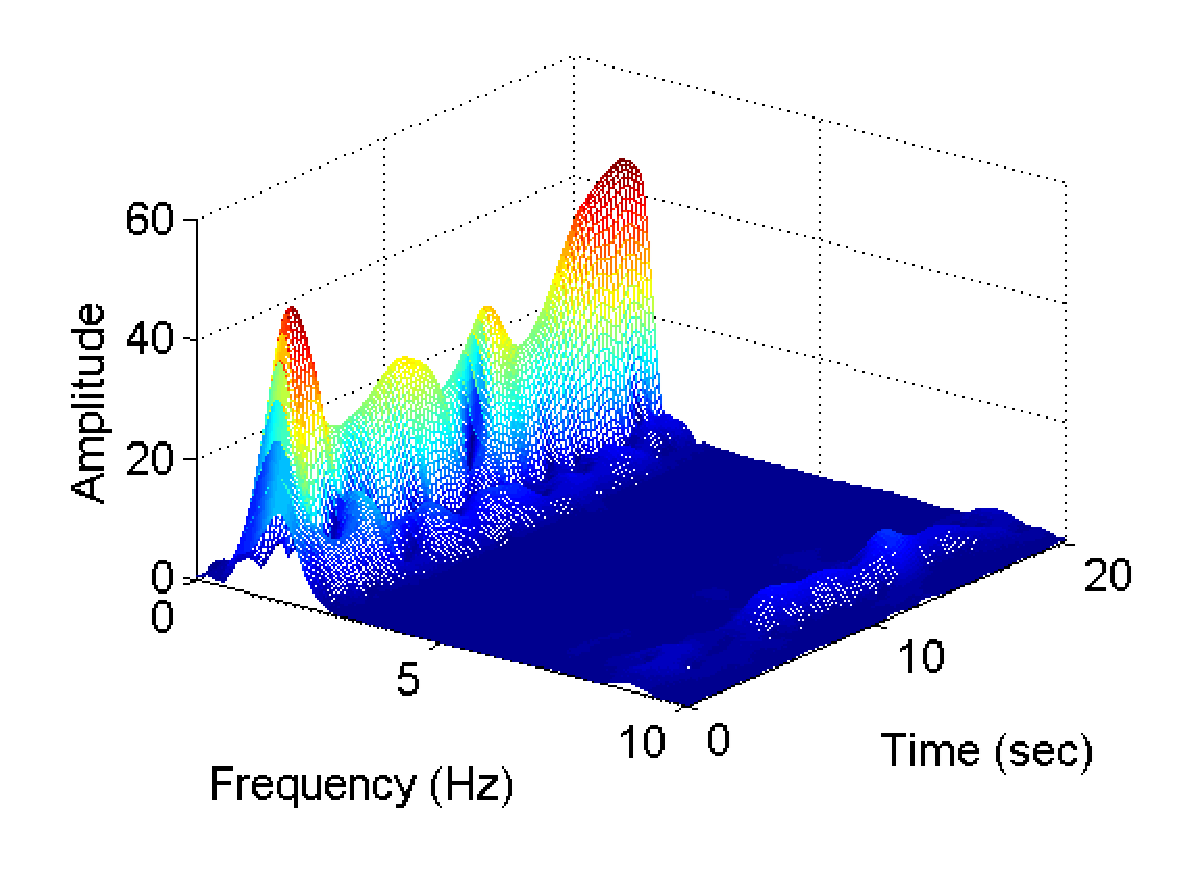
\includegraphics[width=0.45\textwidth] {figure/2-18a.eps}
   \label{fig:2-18a}
 }\hfill
 \subfigure[Spectrogram of the response calculated from the numerical analysis measured]{
   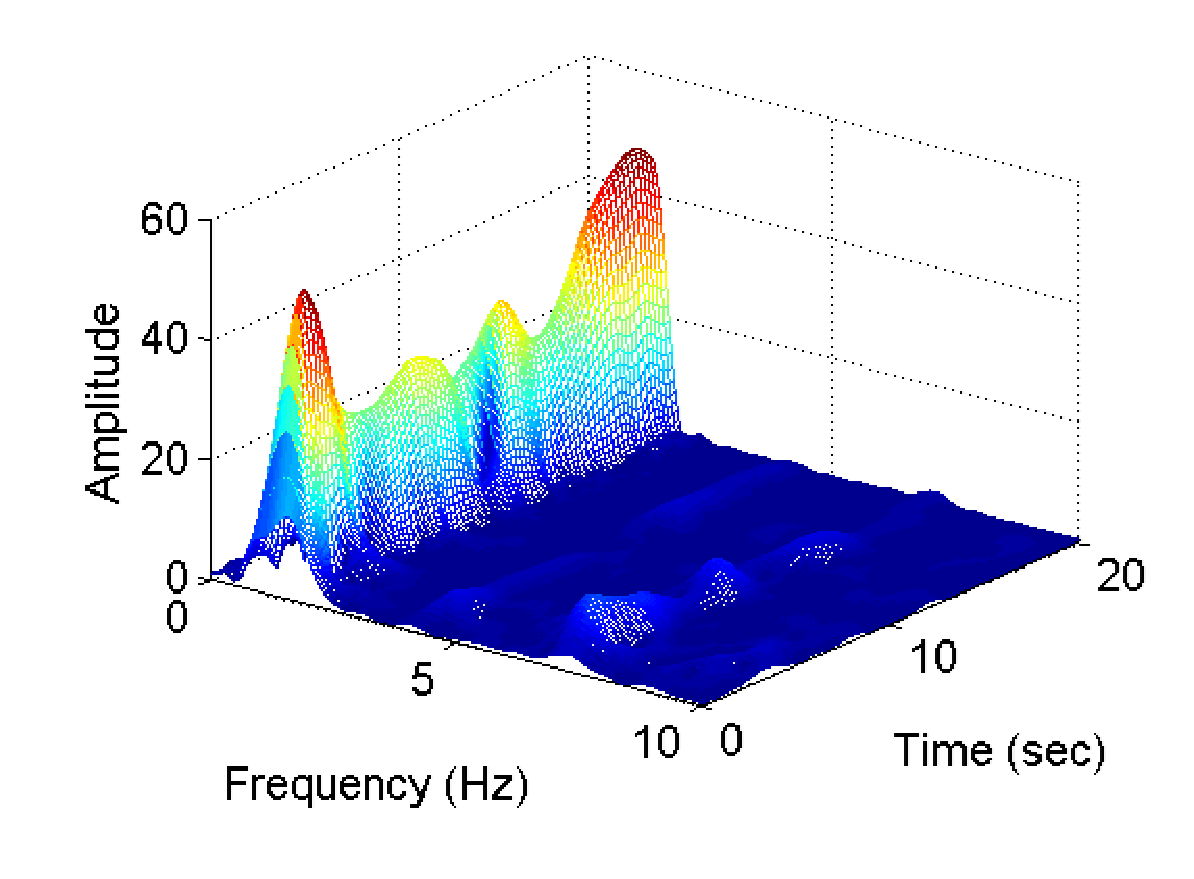
\includegraphics[width=0.45\textwidth] {figure/2-18b.eps}
   \label{fig:2-18b}
 }
 \subfigure[Contour plot of the response measured from the experiment without feedback]{
   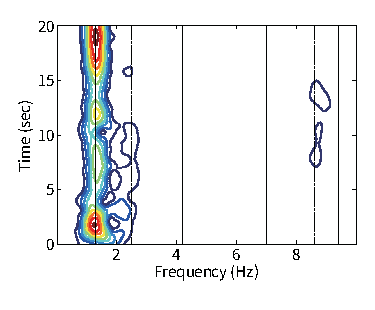
\includegraphics[width=0.45\textwidth] {figure/2-18c.eps}
   \label{fig:2-18c}
 }\hfill
 \subfigure[Contour plot of the response calculated from the numerical analysis measured]{
   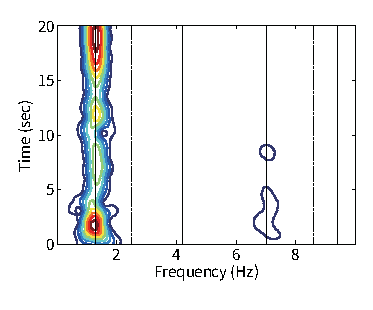
\includegraphics[width=0.45\textwidth] {figure/2-18d.eps}
   \label{fig:2-18d}
 }
\caption{Spectrograms and contour plots of the 4th story acceleration measured from the experiment with feedback and that calculated from the numerical analysis.}
\label{fig:2-18}
\end{figure}

\begin{figure}[ht]
\centering
 \subfigure[Spectrogram of the response measured from the experiment without feedback]{
   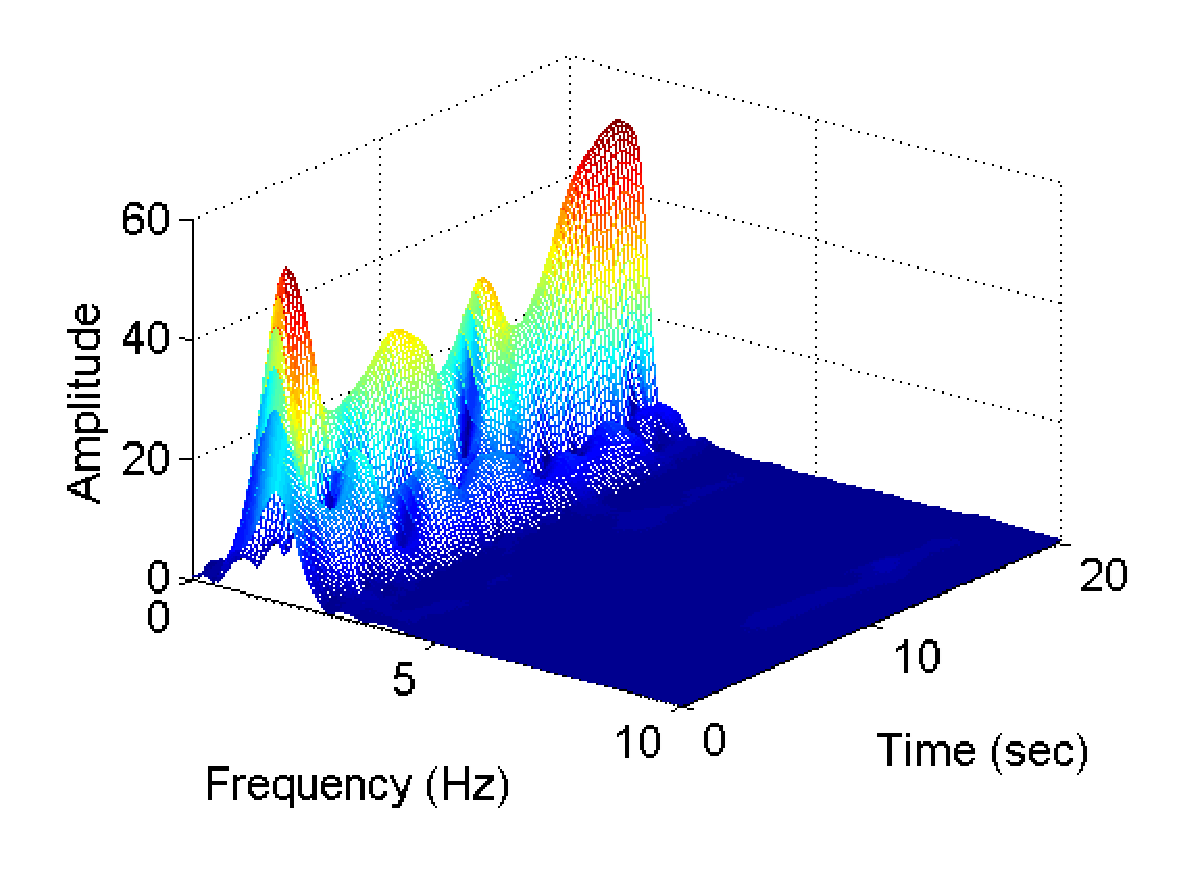
\includegraphics[width=0.45\textwidth] {figure/2-19a.eps}
   \label{fig:2-19a}
 }\hfill
 \subfigure[Spectrogram of the response calculated from the numerical analysis measured]{
   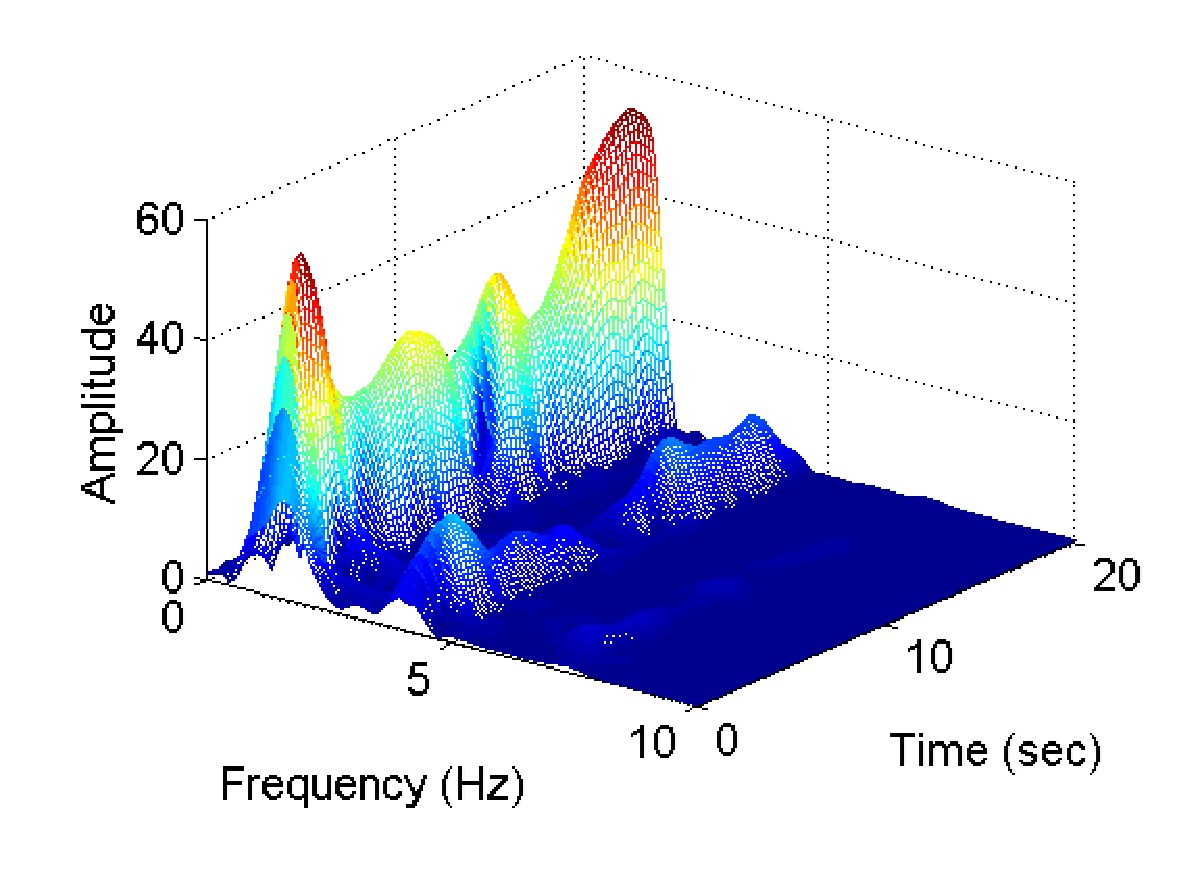
\includegraphics[width=0.45\textwidth] {figure/2-19b.eps}
   \label{fig:2-19b}
 }
 \subfigure[Contour plot of the response measured from the experiment without feedback]{
   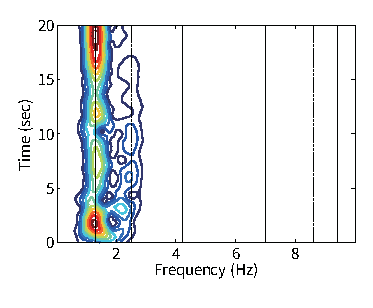
\includegraphics[width=0.45\textwidth] {figure/2-19c.eps}
   \label{fig:2-19c}
 }\hfill
 \subfigure[Contour plot of the response calculated from the numerical analysis measured]{
   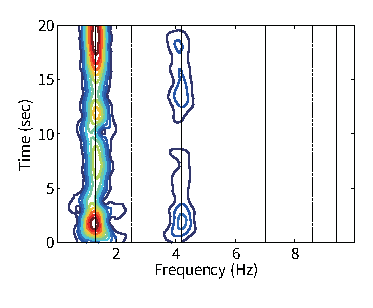
\includegraphics[width=0.45\textwidth] {figure/2-19d.eps}
   \label{fig:2-19d}
 }
\caption{Spectrograms and contour plots of the 5th story acceleration measured from the experiment with feedback and that calculated from the numerical analysis.}
\label{fig:2-19}
\end{figure}

% \clearpage
% \section{Concluding Remarks}
% In this study, a new real-time substructuring technique for the shaking table test was proposed. The proposed substructuring technique adopts the upper part of the whole structure as the experimental substructure, which corresponds to a physical test model. In order to verify the validity and accuracy of the proposed technique, a shaking table test was conducted. The result of the study can be summarized as follows.
% \begin{enumerate}
% \item To reduce the distortion of the interface acceleration, the inverse transfer function of the shaking table was identified and its state space realization was implemented in the shaking table controller.
% \item In this paper, the linear transfer function approach for controlling the motion of a shaking table was considered to experimentally verify the proposed method for a linear experimental part. However, this approach would be inappropriate for a coupled non-linear system leading to experimental instability. Therefore, in such case the controller using the inverse transfer function of shaking table, shown in Fig. 11, would be modified to compensate an experimental instability.
% \item The interface force between the experimental and numerical substructures was obtained using only acceleration measurement and mass information, so that high-capacity loads cell and installation jigs are not required in the experiment. 
% \item The proposed method basing the interface force measurement on acceleration measurements from an experimental substructure is partially available only when the mass distribution is discrete - for example this would be applicable to the TMD as an experimental part. Also, the interface force measurement using force transducers is required to perform the proposed method when wind forces are applied to the experimental substructure.
% \item Experimental results demonstrate that the proposed real-time substructuring technique can reproduce the dynamic behavior of the assumed whole structure.
% \item Unexpected vibration of the experimental substructure can be induced by the feedback of responses including its inherent natural modes and then by the error occurred in calculating the numerical substructure.
% \item It is considered that to minimize the effect of natural modes of an experimental substructure on the substructured system, the structural model as havily-damped as possible would be used as an experimental part.
% \item The proposed technique can be extended to the real-time substructuring technique with the middle part of a whole structure in combination with the conventional substructuring technique employing lower part as the experimental substructure.
% \end{enumerate}


\section{RT-HYTEM of Building controlled by TLD}
\subsection{A Single Story Steel Frame with a TLD}
In this section, experimental verification of the RT-HSTTM is conducted for a single story steel frame with a TLD. First, the conventional TLD-structure interaction model shown in Figure~\ref{fig:3-4a} is tested. Then, the RT-HSTTM shown in Figure~\ref{fig:3-4b}, which incorporates the single story steel frame in the numerical calculation, is performed and the results from the two testing methods are compared to each other.
For the numerical structural model used in RT-HSTTM, the single story steel frame is assumed to be a SDOF mass-damping-spring system. The structure has $0.6m$ of width, $1.0m$ of height and $169.7kg$ of measured floor mass. El Centro, Hachinohe, Mexico city and Northridge earthquake waves were realized by the shaking table and the resulting absolute accelerations of the floor and the shaking table were measured. The system identification was conducted using the measured absolute accelerations. The identified parameters slightly vary according to input earthquake waves. The averaged damping and stiffness coefficients are 14.6$N\cdot s/m$ and $9914.3N/m$, respectively, which correspond to $1.23Hz$ of structural natural frequency. The TLD shown in Figure~\ref{fig:3-4} has the size of $31(cm)\times14(cm)\times20(cm)$. The level of water in the TLD was adjusted to have $3.4cm$ that is theoretically calculated based on the linear wave theory\citep{soong1997passive} for the TLD to have fundamental sloshing frequency tuned to the identified structural natural frequency. As a result, the mass ratio of the TLD to the structure is about $1.3\%$. To confirm whether the numerically calculated frequency of the TLD is modulated to the structural one, the transfer function shown in Figure~\ref{fig:3-5}, from the shaking table acceleration to the shear force by the TLD, was obtained by using the white noise excitation. It is observed in Figure~\ref{fig:3-5} that the TLD has the sloshing frequency of $1.25Hz$ which is very close to the structural natural frequency of $1.23Hz$.

\begin{figure}[!ht]
\centering
\subfigure[Conventional shaking table test]{
   \includegraphics[width=0.8\textwidth] {figure/3-4a.eps}
   \label{fig:3-4a}
 }
 \subfigure[Real-time hybrid shaking table test]{
   \includegraphics[width=0.8\textwidth] {figure/3-4b.eps}
   \label{fig:3-4b}
 }
\caption{TLD-structure interaction experimental system.}
\label{fig:3-4}
\end{figure}

\begin{figure}[!ht]
\centering
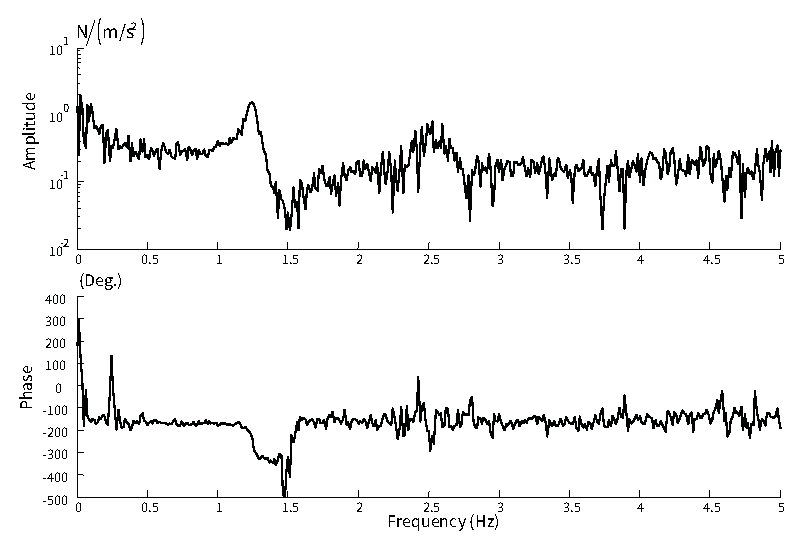
\includegraphics[width=0.8\textwidth] {figure/3-5.eps}
\caption{TLD transfer function from the table acceleration to the base shear force}
\label{fig:3-5}
\end{figure}

At first, the conventional shaking table test shown in Figure~\ref{fig:3-4a} is performed to investigate the seismic response control performance of the TLD. Previously mentioned four earthquake records are scaled to have the peak acceleration of 100 gal and used to excite the TLD-structure system. Figures~\ref{fig:3-6} and \ref{fig:3-7} show the measured structural acceleration responses in the time and frequency domains, respectively. It is observed from Figure~\ref{fig:3-6} that generally acceleration in the latter part of the total response history is significantly reduced. This is typical tendency in the structural response controlled by a tuned mass-type control device, since it makes effect when the structural response is governed by the fundamental mode after initial strong impulse like component has passed. In the response to Mexico-city earthquake excitation, as shown in Figure~\ref{fig:3-7c}, the first peak corresponding to the major frequency component of earthquake itself is not controlled, but the response in the region of the TLD modulation frequency is reduced to nearly zero.

\begin{figure}[!ht]
\centering
 \subfigure[El Centro earthquake]{
   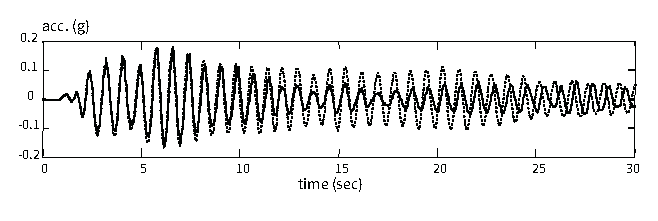
\includegraphics[width=0.8\textwidth] {figure/3-6a.eps}
   \label{fig:3-6a}
 }
 \subfigure[Hachinohe earthquake]{
   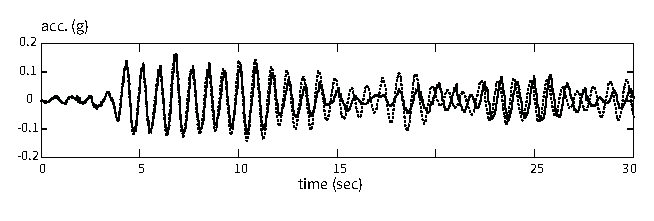
\includegraphics[width=0.8\textwidth] {figure/3-6b.eps}
   \label{fig:3-6b}
 }
 \subfigure[Mexico city earthquake]{
   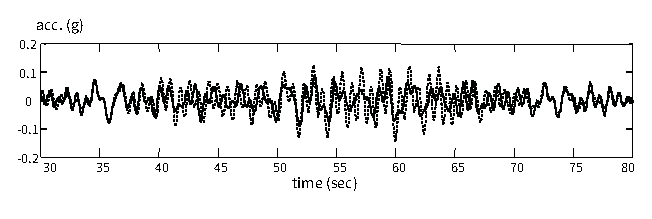
\includegraphics[width=0.8\textwidth] {figure/3-6c.eps}
   \label{fig:3-6c}
 }
 \subfigure[Northridge earthquake]{
   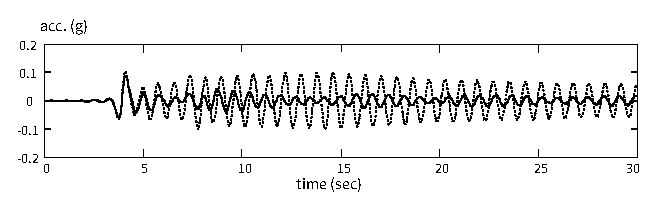
\includegraphics[width=0.8\textwidth] {figure/3-6d.eps}
   \label{fig:3-6d}
 }
\caption{Structural acceleration in the time domain measured from the conventional shaking table test of TLD-structure interaction system (dotted line : without control, solid line : with control)}
\label{fig:3-6}
\end{figure}

\begin{figure}[!ht]
\centering
 \subfigure[El Centro earthquake]{
   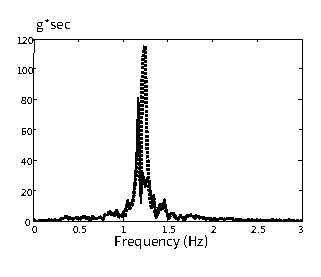
\includegraphics[width=0.45\textwidth] {figure/3-7a.eps}
   \label{fig:3-7a}
 }\hfill
 \subfigure[Hachinohe earthquake]{
   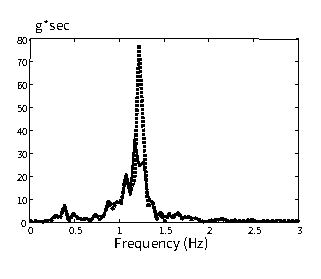
\includegraphics[width=0.45\textwidth] {figure/3-7b.eps}
   \label{fig:3-7b}
 }
 \subfigure[Mexico city earthquake]{
   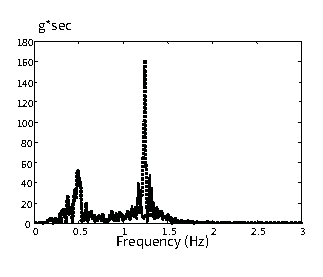
\includegraphics[width=0.45\textwidth] {figure/3-7c.eps}
   \label{fig:3-7c}
 }\hfill
 \subfigure[Northridge earthquake]{
   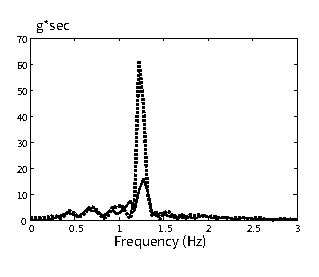
\includegraphics[width=0.45\textwidth] {figure/3-7d.eps}
   \label{fig:3-7d}
 }
\caption{Structural acceleration in the frequency domain measured from the conventional shaking table test of TLD-structure interaction system (dotted line : without control, solid line : with control)}
\label{fig:3-7}
\end{figure}

Then, the RT-HSTTM is applied with the experimental set-up shown in Figure~\ref{fig:3-4b}. For its implementation for the controlled case, the identified structural parameters are reflected in the numerical part expressed by the shaded region in the integrated controller shown in Figure~\ref{fig:3-3}. The continuous filters are converted into discrete ones with a time interval of 0.01 second. Figures~\ref{fig:3-8} and \ref{fig:3-9} compare the controlled accelerations obtained by performing the conventional and the RT-HSTTM in time and frequency domains, respectively. The effectiveness of the RT-HSTTM is verified from the fact that the experimental results from two methods coincide well with each other on the whole. The small discrepancies existing in the controlled responses subjected to El Centro and Hachinohe earthquakes are considered to result from the underestimation of damping coefficients in the numerical structural model since averaged parameters for the four earthquake data were used.

\begin{figure}[!ht]
\centering
 \subfigure[El Centro earthquake]{
   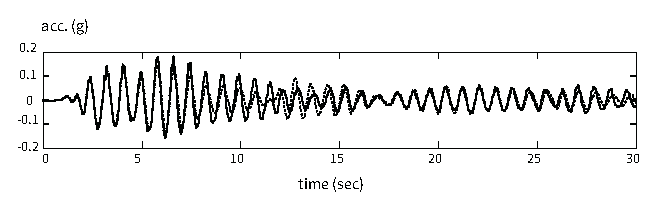
\includegraphics[width=0.8\textwidth] {figure/3-8a.eps}
   \label{fig:3-8a}
 }
 \subfigure[Hachinohe earthquake]{
   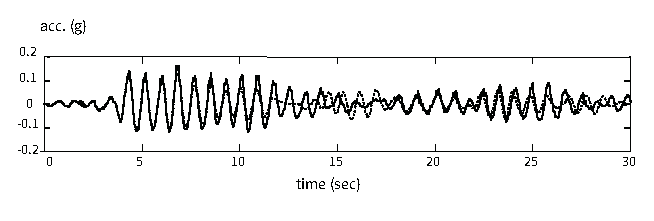
\includegraphics[width=0.8\textwidth] {figure/3-8b.eps}
   \label{fig:3-8b}
 }
 \subfigure[Mexico city earthquake]{
   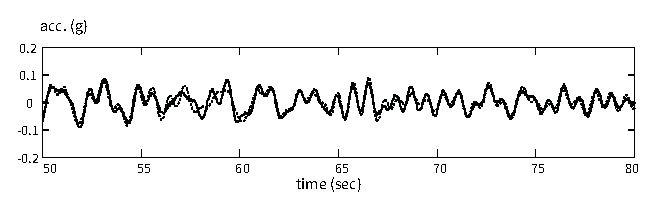
\includegraphics[width=0.8\textwidth] {figure/3-8c.eps}
   \label{fig:3-8c}
 }
 \subfigure[Northridge earthquake]{
   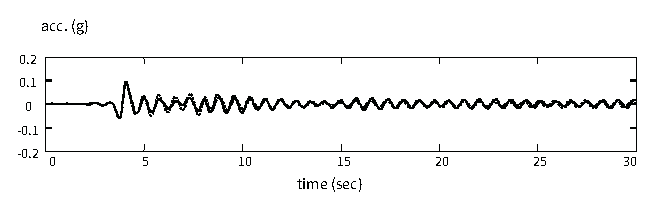
\includegraphics[width=0.8\textwidth] {figure/3-8d.eps}
   \label{fig:3-8d}
 }
\caption{Comparisons of controlled structural accelerations in the time domain
(dotted line : conventional shaking table test, solid line : real-time hybrid shaking table test)
}
\label{fig:3-8}
\end{figure}

\begin{figure}[!ht]
\centering
 \subfigure[El Centro earthquake]{
   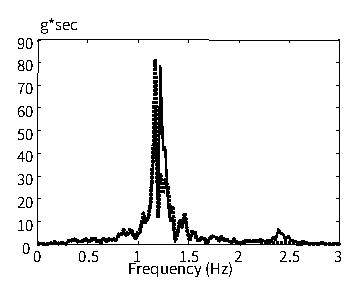
\includegraphics[width=0.45\textwidth] {figure/3-9a.eps}
   \label{fig:3-9a}
 }\hfill
 \subfigure[Hachinohe earthquake]{
   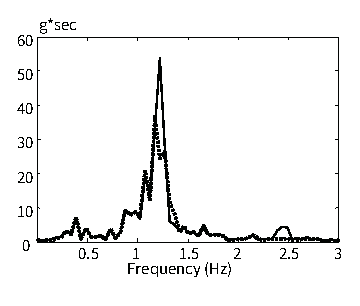
\includegraphics[width=0.45\textwidth] {figure/3-9b.eps}
   \label{fig:3-9b}
 }
 \subfigure[Mexico city earthquake]{
   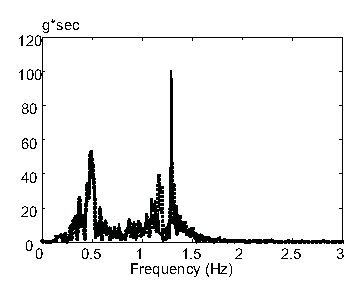
\includegraphics[width=0.45\textwidth] {figure/3-9c.eps}
   \label{fig:3-9c}
 }\hfill
 \subfigure[Northridge earthquake]{
   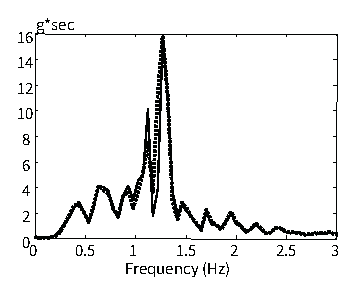
\includegraphics[width=0.45\textwidth] {figure/3-9d.eps}
   \label{fig:3-9d}
 }
\caption{Comparisons of controlled structural accelerations in the frequency domain (dotted line : conventional shaking table test, solid line : real-time hybrid shaking table test)}
\label{fig:3-9}
\end{figure}

\clearpage
\subsection{Three Story Structure with a TLD}
The control performance of a TLD installed in a three story structure is investigated by using the RT-HSTTM. The structure is assumed to be a three story shear-type model, which has identical story properties as follows; $m_{i}=128.8kg$, $c_{i}=13.52N\cdot s/m$, $k_{i}=33908N/m$ for $i=1,2,3$. The structure has natural frequencies of $1.15Hz$, $3.22Hz$ and $4.65Hz$. The TLD discussed in the previous section is used and its water level is modulated to $4.6cm$ in order for the TLD to have sloshing frequency of $1.15Hz$. As a result, the mass ratio of the TLD to the structure is about $2\%$. The four earthquake waves used for the excitation of the single story steel frame were scaled to have peak acceleration of $40gal$. The uncontrolled structural responses were obtained by removing the feed back loop of the TLD-generated interacting force, which causes the numerical structural model to be excited only by the base earthquake motion. 
Figures~\ref{fig:3-10} and \ref{fig:3-11} compare the uncontrolled and controlled accelerations of the third story in time and frequency domains, respectively, which is realized by the shaking table through the RT-HSTTM. It is observed that the structural accelerations are significantly reduced by the TLD, especially in the region of the fundamental frequency. Table~\ref{tab:3-1} indicates that the acceleration is reduced by $4-30\%$ in peak and by $18-60\%$ in RMS responses. It is also identified in Figure~\ref{fig:3-11d} that the TLD lessens the additional second mode response of the structure. Figure~\ref{fig:3-12} shows the typical sloshing and slamming behaviors of the water in the TLD tanks during the experiment, which occur in the small and large amplitude of the water motion, respectively\citep{yalla2001liquid}.

\begin{figure}[!ht]
\centering
 \subfigure[El Centro earthquake]{
   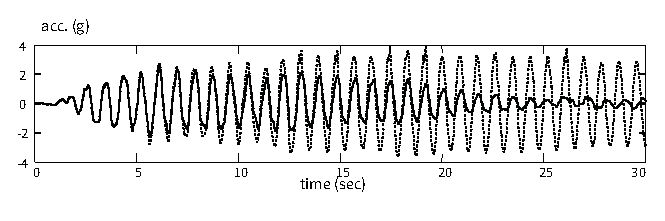
\includegraphics[width=0.8\textwidth] {figure/3-10a.eps}
   \label{fig:3-10a}
 }
 \subfigure[Hachinohe earthquake]{
   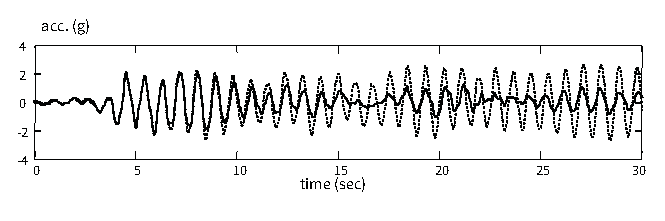
\includegraphics[width=0.8\textwidth] {figure/3-10b.eps}
   \label{fig:3-10b}
 }
 \subfigure[Mexico city earthquake]{
   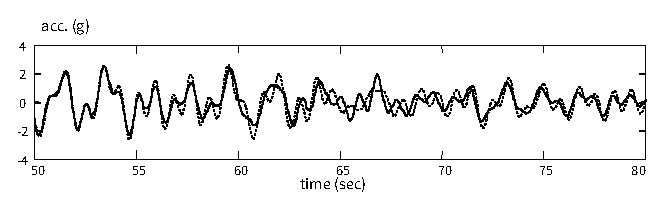
\includegraphics[width=0.8\textwidth] {figure/3-10c.eps}
   \label{fig:3-10c}
 }
 \subfigure[Northridge earthquake]{
   \includegraphics[width=0.8\textwidth] {figure/3-10d.eps}
   \label{fig:3-10d}
 }
\caption{Absolute accelerations in the time domain, measured from the top story of MDOF structure with a TLD by the real-time hybrid shaking table test (dotted line : without control, solid line : with control))
}
\label{fig:3-10}
\end{figure}

\begin{figure}[!ht]
\centering
 \subfigure[El Centro earthquake]{
   \includegraphics[width=0.45\textwidth] {figure/3-11a.eps}
   \label{fig:3-11a}
 }\hfill
 \subfigure[Hachinohe earthquake]{
   \includegraphics[width=0.45\textwidth] {figure/3-11b.eps}
   \label{fig:3-11b}
 }
 \subfigure[Mexico city earthquake]{
   \includegraphics[width=0.45\textwidth] {figure/3-11c.eps}
   \label{fig:3-11c}
 }\hfill
 \subfigure[Northridge earthquake]{
   \includegraphics[width=0.45\textwidth] {figure/3-11d.eps}
   \label{fig:3-11d}
 }
\caption{Absolute accelerations in the frequency domain, measured from the top story of MDOF structure with a TLD by the real-time hybrid shaking table test (dotted line : without control, solid line : with control)}
\label{fig:3-11}
\end{figure}

\begin{figure}[!ht]
\centering
 \subfigure[Sloshing of TLD]{
   \includegraphics[width=0.45\textwidth] {figure/3-12a.eps}
   \label{fig:3-12a}
 }\hfill
 \subfigure[Slamming of TLD]{
   \includegraphics[width=0.45\textwidth] {figure/3-12b.eps}
   \label{fig:3-12b}
 }
\caption{Behaviors of a TLD under the earthquake motion}
\label{fig:3-12}
\end{figure}

\begin{table}[ht]
\centering
\begin{tabularx}{\textwidth}{b|s|s|s|s}
\toprule[1pt]\midrule[0.3pt]
Responses$(g)$&El Centro&Hachinohe&Mexico City&Northridge\\ \midrule[0.3pt]
\textit{Peak acceleration}&&&&\\
Uncontrolled& 3.85&2.71&2.63&1.34\\
Controlled& 2.69&2.19&252&1.34\\
\textit{RMS acceleration}&&&&\\
Uncontrolled&1.91&1.36&0.54&0.33\\
Controlled&0.74&0.66&0.45&0.27\\ \bottomrule
\end{tabularx}
\caption{Uncontrolled and controlled responses of a combined TLD–MDOF structure system}
\label{tab:3-1}
\end{table}

% \section{Concluding Remarks}
% In this study, a real-time hybrid shaking table test was conducted to verify the seismic control performance of the TLD installed in the building structures. The TLD installed at the top floor of the structure is physically tested, and simultaneously numerical calculation is carried out for the assumed analytical structural model. Comparison between the structural responses obtained by the RT-HSTTM and the conventional shaking table test of a single story steel frame with TLD indicates that the performance of the TLD can be accurately evaluated using the RT-HSTTM without the physical structural model. Finally, the uncontrolled and TLD-controlled structural responses of a three story structure are obtained by the RT-HSTTM in both time and frequency domains, showing that TLD can effectively mitigate the seismic responses of building structures and the RT-HSTTM can reproduce the dynamic behavior of TLD-structure interaction systems for both the uncontrolled and controlled case. The RT-HSTTM can be also applied to the performance evaluation of tuned liquid column damper which has strong inherent nonlinearity.

\section{RT-HYTEM of Building controlled by TLCD}
\subsection{A Single Story Steel Frame with a TLCD}
At first, the conventional shaking table test with this TLCD shown in Figure~\ref{fig:4-4a} is performed to reduce the structural response. Two earthquake records with the maximum acceleration of $100gal$ due to the shaking table performance are used to excite the TLCD-structure system with control case. Then, the hybrid shaking table test is conducted with the experimental set-up shown in Figure~\ref{fig:4-4b}. For its experimental implementation, the identified structural parameters are reflected in the numerical part expressed by the shaded region in the integrated controller shown in Figure~\ref{fig:4-3}. The continuous filters in the figure are converted into discrete ones with a time step of 0.01 sec in actual implementation of the experiment. Figure~\ref{fig:4-5} compare the controlled accelerations experimentally measured by implementing the conventional and the real-time hybrid shaking table tests in both time and frequency domain, respectively. The validity of the real-time hybrid shaking table test performed in this paper is verified from the fact that the experimental results from two methods well coincide with each other on the whole.

\begin{figure}[!ht]
\centering
 \subfigure[El Centro Earthquake(time domain)]{
   \includegraphics[width=0.45\textwidth] {figure/4-5a.eps}
   \label{fig:4-5a}
 }\hfill
 \subfigure[El Centro Earthquake(frequency domain)]{
   \includegraphics[width=0.45\textwidth] {figure/4-5b.eps}
   \label{fig:4-5b}
 }
 \subfigure[Kobe Earthquake(time domain)]{
   \includegraphics[width=0.45\textwidth] {figure/4-5c.eps}
   \label{fig:4-5c}
 }\hfill
 \subfigure[Kobe Earthquake(frequency domain)]{
   \includegraphics[width=0.45\textwidth] {figure/4-5d.eps}
   \label{fig:4-5d}
 }
\caption{Comparisons between the results from the conventional testing method(dotted line) and those from the RT-HSTTM(solid line) for the controlled response}
\label{fig:4-5}
\end{figure}

% \section{Concluding Remarks}
% In this study, a real-time hybrid shaking table test was conducted to verify the seismic control performance of the TLCD installed in the building structures. The TLCD installed at the top floor of the structure is physically tested, and simultaneously numerical calculation is carried out for the assumed analytical structural model. Comparison between the structural responses obtained by the RT-HSTTM and the conventional shaking table test of a single story steel frame with TLCD indicates that the performance of the TLCD can be accurately evaluated using the RT-HSTTM without the physical structural model.

\section{RT-HYTEM of Building controlled by TLMD}
\section{Conventional Testing Method}
\subsection{Experimental installation}

The test on a scaled-down TLMD building model shown in Figure~\ref{fig:5-3} was performed to experimentally verify the control performance of a proposed TLMD.

In order to experimentally describe the dynamic behavior of a building model, the moving mass of $4250 kg$ was mounted on guide rails. Also, the springs that connect the moving mass to both the actuator and the retaining block were devised to characterize the behavior of the stiffness of a building model, as shown in Figure~\ref{fig:5-4}. In the figure, $m_{s}$, $c_{s}$ and $k_{1} + k_{2} = k_{s}$ represent the mass, damping coeffi cient and stiffness of a building model, respectively. $x_{1}$, $x_{2}$ and $x_{3}$ denote the displacement and acceleration of a building model, dynamic actuator and TLMD, respectively. Ten springs with the stiffness of $11,000 N/m$ for each one were used for the case of a test in the TMD control direction, and eight springs with $8800 N/m$ for each one for the case of a test in the TLCD control direction.

\begin{figure}[ht]
\centering
\includegraphics[width=0.8\textwidth] {figure/5-2.eps}
\caption{Photograph of the manufactured TLMD}
\label{fig:5-2}
\end{figure}

\begin{figure}[ht]
\centering
\includegraphics[width=0.8\textwidth] {figure/5-3.eps}
\caption{Experimental TLMD-building model}
\label{fig:5-3}
\end{figure}

\begin{figure}[ht]
\centering
\includegraphics[width=0.8\textwidth] {figure/5-4.eps}
\caption{Conceptual view of experimental set-up}
\label{fig:5-4}
\end{figure}

It is noted from Figure~\ref{fig:5-5} that the mass of a building model is excited by the force transmitted by the spring, $k_{2}$, through the displacement of an actuator, $x_{2}$. Accordingly, the motion of a building model is expressed by

\begin{equation}\label{eq:5-3}
m_{s}\ddot{x}_{1}+c_{s}\dot{x}_{1}+k_{1}x_{1}-k_{2}\left(x_{2}-x_{1}\right)=0
\end{equation}

In this case, the displacement of an actuator, $x_{2}$, is given by

\begin{equation}\label{eq:5-4}
x_{2}=A sin \left(2 \pi f_{e} t \right)
\end{equation}

where $A$ and $f_{e}$ are the excitation amplitude and frequency of an actuator, respectively.

Finally, the equation of motion of a building model is obtained by substituting Eq.~\eqref{eq:5-4} into Eq.~\eqref{eq:5-3}.

\begin{equation}\label{eq:5-5}
m_{s}\ddot{x}_{1}+c_{s}\dot{x}_{1}+k_{s}x_{1} = k_{2}A sin \left(2 \pi f_{e} t \right)
\end{equation}

\begin{figure}[!ht]
\centering
\subfigure[Mass]{
   \includegraphics[width=0.45\textwidth] {figure/5-5a.eps}
   \label{fig:5-5a}
 }
 \subfigure[Actuator]{
   \includegraphics[width=0.45\textwidth] {figure/5-5b.eps}
   \label{fig:5-5b}
 }
\caption{Free-body diagram of a building model.}
\label{fig:5-5}
\end{figure}

\subsection{Test results}
In this test, the building model was excited by a dynamic actuator installed on the strong wall. Maximum excitation displacement of the dynamic actuator was set to be 4 mm. Harmonic waves with the frequency interval of 0.05 Hz from 0.1 to 3.0 Hz were imposed on the moving mass of a building model by the actuator. Especially, harmonic waves with the frequency interval of 0.01 Hz were excited to the moving mass in the vicinity of its natural frequencies during 200s. Then, the steady-state response of the moving mass was obtained in each excitation frequency.

First, the test was performed in the TMD control direction. In this case, the frequency of structural model was set to 0.82 Hz by connecting springs with the stiffness of 110,000 N/m to the structural model with the mass of 4,250 kg. Figures~\ref{fig:5-6} and \ref{fig:5-7} show the displacement and acceleration response of the SDOF structure in the frequency domain, respectively. It is verified that the displacement response of the SDOF structure was reduced by $82\%$ for the case in the TMD control direction. The displacement control performance index of a TMD is 0.18, as shown in Figure~\ref{fig:5-6}. Also, the acceleration response of the SDOF structure was reduced by $80\%$, and the acceleration control performance index of a TMD is 0.20, as shown in Figure~\ref{fig:5-7}. Figures~\ref{fig:5-6} and \ref{fig:5-9} show the displacement and acceleration response of the SDOF structure in the time domain, respectively. Also, the response of the SDOF structure tuned by the TMD is considerably reduced at a resonance frequency of 0.82 Hz, as shown in Figure~\ref{fig:5-8}.

Then, the test was carried out in the TLCD control direction. In this case, the frequency of structural model was tuned to 0.73 Hz by connecting springs with the stiffness of 88,000 N/m to the moving mass of 4,250 kg. Figures~\ref{fig:5-9} and \ref{fig:5-10} show the displacement and acceleration response of the SDOF structure in the frequency domain, respectively. It is observed that the displacement response of the SDOF structure was reduced by $71\%$ for the case in the TLCD control direction. The displacement control performance index of a TLCD is 0.29, as shown in Figure~\ref{fig:5-9}. Also, the acceleration response of the SDOF structure was reduced by $70\%$, and the acceleration control performance index of a TLCD is 0.30, as shown in Figure~\ref{fig:5-10}. Also, the displacement response of the SDOF structure tuned by TLCD is considerably reduced at a resonance frequency of 0.73 Hz, respectively, as shown in Figure~\ref{fig:5-11}.

\begin{figure}[ht]
\centering
\includegraphics[width=0.8\textwidth] {figure/5-6.eps}
\caption{Displacement in the frequency domain (TMD direction)}
\label{fig:5-6}
\end{figure}

\begin{figure}[ht]
\centering
\includegraphics[width=0.8\textwidth] {figure/5-7.eps}
\caption{Acceleration in the frequency domain (TMD direction)}
\label{fig:5-7}
\end{figure}

\begin{figure}[ht]
\centering
\includegraphics[width=0.8\textwidth] {figure/5-8.eps}
\caption{Displacement in the time domain (TMD direction, 0.82 Hz)}
\label{fig:5-8}
\end{figure}

\begin{figure}[ht]
\centering
\includegraphics[width=0.8\textwidth] {figure/5-9.eps}
\caption{Displacement in the frequency domain (TLCD direction)}
\label{fig:5-9}
\end{figure}

\begin{figure}[ht]
\centering
\includegraphics[width=0.8\textwidth] {figure/5-10.eps}
\caption{Acceleration in the frequency domain (TLCD direction)}
\label{fig:5-10}
\end{figure}

\begin{figure}[ht]
\centering
\includegraphics[width=0.8\textwidth] {figure/5-11.eps}
\caption{Displacement in the time domain (TMD direction, 0·73 Hz)}
\label{fig:5-11}
\end{figure}

\subsection{RT-HYTEM Test results}
A TLMD is excited by uniaxial shaking table. Shear type load cell and acceleration sensors are attached on the shaking table to monitor the dynamic characteristic of the shaking table. The vibration control and data acquisition are conducted using a real-time digital signal processor. The main task of the data acquisition board is data conversion; it converts the measured shear force and acceleration to the digital data, and converts the reference signal computed by the control program MATLAB to the analog data. An eight-channel data acquisition system was adopted which uses a NI DAQcard-6036E board and a BNC-2110 BNC cable connector. At the real-time hybrid test, the control performance results of the TLMD were evaluated. In this test, the checking point is whether the natural frequencies of the TLMD in the TMD and TLCD control direction were seen at 0.82 and 0.73 Hz, respectively. Then, control performance of the bidirectional TLMD will be evaluated.

First, the test was performed in the TMD control direction. Figures~\ref{fig:5-19} and \ref{fig:5-20} show the displacement and acceleration response in the frequency domain, respectively. It is observed that the displacement response of the shaking table was reduced by 78\% for the case in the TMD control direction. The displacement control performance index of a TMD is 0.22, as shown in Figure~\ref{fig:5-19}. Also, the acceleration response of the shaking table was reduced by 78\%, as shown in Figure~\ref{fig:5-20}. Figure~\ref{fig:5-21} shows the displacement in the time domain. The response of the shaking table is considerably reduced by 78\% at a resonance frequency of 0.82 Hz.

Then, the test was performed in the TLCD control direction. Figures~\ref{fig:5-22} and \ref{fig:5-23} show the displacement and acceleration response of the shaking table in the frequency domain, respectively. It is observed that the displacement response was reduced by 71\% for the case in the TLCD control direction, and the acceleration response reduced by 70\%. Also, the displacement and acceleration response of the shaking table are considerably reduced at a resonance frequency of 0.73 Hz, respectively, as shown in Figure~\ref{fig:5-24}.

\begin{figure}[ht]
\centering
\includegraphics[width=0.8\textwidth] {figure/5-19.eps}
\caption{Displacement in the frequency domain by the hybrid test (TMD direction)}
\label{fig:5-19}
\end{figure}

\begin{figure}[ht]
\centering
\includegraphics[width=0.8\textwidth] {figure/5-20.eps}
\caption{Acceleration in the frequency domain by the hybrid test (TMD direction)}
\label{fig:5-20}
\end{figure}

\begin{figure}[ht]
\centering
\includegraphics[width=0.8\textwidth] {figure/5-21.eps}
\caption{Displacement in the time domain by the hybrid test (TMD direction, 0.83 Hz)}
\label{fig:5-21}
\end{figure}

\begin{figure}[ht]
\centering
\includegraphics[width=0.8\textwidth] {figure/5-22.eps}
\caption{Displacement in the frequency domain by the hybrid test (TLCD direction)}
\label{fig:5-22}
\end{figure}

\begin{figure}[ht]
\centering
\includegraphics[width=0.8\textwidth] {figure/5-23.eps}
\caption{Acceleration in the frequency domain by the hybrid test (TLCD direction)}
\label{fig:5-23}
\end{figure}

\begin{figure}[ht]
\centering
\includegraphics[width=0.8\textwidth] {figure/5-24.eps}
\caption{Displacement in the time domain by the hybrid test (TLCD direction, 0.73 Hz)}
\label{fig:5-24}
\end{figure}

\subsection{Comparisons of test results}

In order to compare the control performances of the TLMD at the RT-HYTEM and conventional method, $J_{1}$, $J_{2}$, $J_{3}$, $J_{4}$, are represented by

\begin{align}
J_{1}&=\frac{\text{max} \left[x_{c}(t) \right]}{\text{max} \left[x_{u}(t) \right]} \label{eq:5-14} \\
J_{2}&=\frac{\text{max} \left[\ddot{x}_{c}(t) \right]}{\text{max} \left[\ddot{x}_{u}(t) \right]} \label{eq:5-15} \\
J_{3}&=\frac{\text{rms} \left[x_{c}(t) \right]}{\text{rms} \left[x_{u}(t) \right]} \label{eq:5-16} \\
J_{4}&=\frac{\text{rms} \left[\ddot{x}_{c}(t) \right]}{\text{rms} \left[\ddot{x}_{u}(t) \right]} \label{eq:5-17}
\end{align}

where $x_{u}$ and $x_{c}$ are uncontrolled displacement and controlled displacement, respectively. $\ddot{x}_{u}$ and $\ddot{x}_{c}$ are uncontrolled acceleration and controlled acceleration, respectively.

Tables~\ref{tab:5-4} and \ref{tab:5-5} show the control performance of the TLMD through the conventional test and hybrid test, respectively. According to the test result in the TLCD control direction, the errors of $J_{1}$ or $J_{2}$ between the results of conventional test and hybrid test were all 0.01, but the errors of $J_{3}$ or $J_{4}$ between the conventional test and hybrid test were 0.03 and 0.04, respectively. In the TMD control direction, the errors of $J_{1}$, $J_{2}$, $J_{3}$, $J_{4}$ between the conventional test and hybrid test were 0.04, 0.02, 0.06, 0.06, respectively.

\begin{table}[ht]
\centering
\begin{tabularx}{\textwidth}{@{}XXXX@{}}
\toprule[1pt]\midrule[0.3pt]
&& TMD & TLCD\\ \hline
Effective mass && $1.8\%$ & $0.8\%$\\
Peak value & $J_{1}$ & 0.18 & 0.29\\
& $J_{2}$ & 0.20 & 0.30\\
RMS value & $J_{3}$ & 0.17 & 0.28\\
& $J_{4}$ & 0.17 & 0.27\\
\bottomrule
\end{tabularx}
\caption{Control performance of real-structure test}
\label{tab:5-4}
\end{table}

\begin{table}[ht]
\centering
\begin{tabularx}{\textwidth}{@{}XXXX@{}}
\toprule[1pt]\midrule[0.3pt]
&& TMD & TLCD\\ \hline
Effective mass && $1.8\%$ & $0.8\%$\\
Peak value & $J_{1}$ & 0.22 & 0.30\\
& $J_{2}$ & 0.22 & 0.29\\
RMS value & $J_{3}$ & 0.23 & 0.31\\
& $J_{4}$ & 0.23 & 0.31\\
\bottomrule
\end{tabularx}
\caption{Control performance of real-time hybrid test}
\label{tab:5-5}
\end{table}

\begin{figure}[ht]
\centering
\includegraphics[width=0.8\textwidth] {figure/5-25.eps}
\caption{Uncontrolled displacement comparison in the time domain between the real-structure test and real-time hybrid test (TMD direction)}
\label{fig:5-25}
\end{figure}

% \section{CONCLUDING REMARKS}
% The bidirectional control performance of the TLMD was confi rmed through the conventional test and real-time hybrid test. First, resonance frequencies in the TMD and TLCD control direction were confirmed at 0.82 and 0.73 Hz. In the TMD control direction ($x-$direction), 80\% of the uncontrolled peak response of the target structure was removed by a TLMD. Also, in the TLCD control direction ($y-$direction), 70\% was removed by a TLMD.

% The control performances of the TLMD were checked and compared through the two testing methods. In the TLCD and TMD control direction, the errors of the peak values between the conventional test and hybrid test were 0.01 and 0.02-0.04, respectively. Also, the errors of RMS values between the conventional test and hybrid test were up to 0.06. However, tuning error and outside environment are thought as the causes of the differences. The error of the convergence times reaching to the peak value as shown in Figure~\ref{fig:5-25}. This is caused by the minute error of the mass, stiffness and damping ratio at the numerical analysis, which was thought as either reason.

% As showing the similar results of the two tests, the outstanding performance of the two-way TLMD was verified. Also, the results show that the RT-HYTEM, which does not require the physical structural model but with simple installation, as well as the conventional method, can accurately evaluate the control performance of a control device.








\section{RT-HYTEM Verification of Semi-actively Controlled Building Structure Equipped with Full-scale MR Damper}
\subsection{Integrated Controller of the Numerical Substructure and UTM}

The numerical substructure and the approximated ITRF explained above are incorporated into the control computer as an integrated controller to implement RT-HYTEM, as shown by the shaded area in Figure~\ref{fig:8-7}. First, when the constant current sent from the signal generator for the passive control test and the calculated current of semi-active control algorithms sent from the analog output for the semi-active control test are applied to the MR damper, the control force proportional to the magnitude of the current signal is developed and transferred to the UTM. The drift response, $x_{1}(t)$, of the first story where the MR damper is positioned is then calculated from the numerical substructure, given by Eq.~\eqref{eq:8-8}, with two inputs: the control force, $f_{e}(t)$, measured from the load cell attached to the UTM and the ground input acceleration, $\ddot{x}_{g}(t)$ given by the user. The motion of the UTM is driven by the controller using the ITRF, represented by Eq~\eqref{eq:8-12}, so that the UTM itself operates as the first story where the MR damper is located, and excites the MR damper that should be physically tested. In the actual experimental implementation of RT-HYTEM, the continuous filters shown in Figure~\ref{fig:8-7} are converted into discrete filters with a time interval of 0.01s, while MATLAB \textit{Simulink}\citep{simulink2009version} and \textit{Real-Time Windows Target}\citep{targetuser} are used as the control system.

\subsection{Experimental Verification for Simple Bouc-Wen Model}

RT-HYTEM with a sinusoidal wave excitation is carried out to investigate the hysteretic behavior of the MR damper and to verify the RT-HYTEM experimentally implemented in this study. A current of 0 A is applied to the MR damper and a sine wave with a frequency of 0.52 Hz, which corresponds to the fundamental frequency of the numerical substructure, and with an amplitude of $5m/s^{2}$ is used as the ground input acceleration as shown in Figure~\ref{fig:8-7}.

\begin{figure}[H]
\centering
\includegraphics[width=0.8\textwidth] {figure/8-7.eps}
\caption{Integrated controller for implementing RTHTM.}
\label{fig:8-7}
\end{figure}

Parametric identification is then performed to find the numerical model of the MR damper on the basis of the experimentally measured hysteretic loop. The Bouc-Wen model is widely used for modeling various hysteretic loops\citep{wen1976method}. The control force by the MR damper can also be specified using this model. The force described by this model is represented by:

\begin{equation}\label{eq:8-13}
f_{MR}(t) = \alpha z(t) + c_{MR}\dot{x}_{1}(t) + k_{MR}x_{1}(t) + f_{0}
\end{equation}

where, $k_{MR}$ and $c_{MR}$ are the stiffness and viscosity of the MR damper; $f_{0}$ the initial friction force; $z$ a dimensionless valuable introduced to describe the hysteresis; and $\alpha$ a variable that regulates the effect of $z$ on $f_{MR}(t)$ which depends on the magnetic field; $z$ is given by the following differential equation.

\begin{equation}\label{eq:8-14}
\dot{z}(t) = -\gamma |\dot{x}_{1}(t)| z(t) |z(t)|^{n-1}-\beta\dot{x}_{1}(t)|z(t)|^{n}+A\dot{x}_{1}(t)
\end{equation}

where $\gamma$, $\beta$, $A$ and the superscript $n$ are the coefficients determining the shape of the hysteretic curve.

The eight parameters in Eqs.~\eqref{eq:8-13} and \eqref{eq:8-14} ($\alpha$, $c_{MR}$, $k_{MR}$, $f_{0}$, $\gamma$, $n$, $\beta$ and $A$) are identified using
least-squares optimization to minimize the performance index defined as:

\begin{equation}\label{eq:8-15}
J\left(\matr{p}\right) = \sum_{k=1}^{N}\left[f_{e}\left(k\cdot\Delta T \right) - f_{MR}\left(\matr{p}, k\cdot\Delta t \right)\right]^{2}
\end{equation}

where $f_{e}\left(k\cdot\Delta t\right)$ represents the force data measured at the $k-$th sampling time; $\matr{p}$ the $1\times8$ vector of the identification parameter, $\left\{ \alpha, c_{MR}, k_{MR}, f_{0}, \gamma, n, \beta, A \right\}$; and $f_{MR}\left(\matr{p},k\cdot\Delta t\right)$ the force obtained at the $k-$th calculating time from Eq.~\eqref{eq:8-13} and \eqref{eq:8-14} using the parameter $\matr{p}$.

This procedure is carried out using MATLAB subroutines\citep{coleman1999optimization}, and the identified parameters are given by:

\begin{equation}\label{eq:8-16}
\begin{aligned}
\alpha &=13288.130 (N/m), & c_{MR} = 81418.582 (N\cdot s/m), \\
k_{MR} &=16647.456 (N/m), & f_{0} = 6.10 (N), \\
n &= 3.0581, & \gamma = 471409.377 (m^{-n}),\\
\beta&=335518.804 (m^{-n}), & A=497.295
\end{aligned}
\end{equation}

A comparison between the calculated and experimental responses is provided in Figure~\ref{fig:8-8}. The displacement and velocity in Figures~\ref{fig:8-8b} and ~\ref{fig:8-8c} correspond to the first-story drift and velocity responses, respectively. The Bouc-Wen model represents the force-displacement and the force-velocity hysteretic behaviors of the damper well.

\begin{figure}[H]
\centering
\subfigure[time history of force]{
   \includegraphics[width=0.9\textwidth] {figure/8-8a.eps}
   \label{fig:8-8a}
}
\subfigure[force-displacement relation]{
   \includegraphics[width=0.45\textwidth] {figure/8-8b.eps}
   \label{fig:8-8b}
}
\subfigure[force-velocity relation]{
   \includegraphics[width=0.42\textwidth] {figure/8-8c.eps}
   \label{fig:8-8c}
}
\caption{Comparison between calculated and experimentally measured responses for the Bouc-Wen model.}
\label{fig:8-8}
\end{figure}

The RT-HYTEM implemented in this study is verified by experiment using the excitation of historical seismic measurements. Four different records of earthquake acceleration measurements taken at El Centro, Hachinohe, Kobe, and Northridge are used as ground input acceleration in Figure~\ref{fig:8-7} by multiplying them by 0.05. Also, the current of 0 [A] is applied to an MR damper in the same manner as the sinusoidal excitation test above. In addition to the measurement of the control force produced by an MR damper, given by Eqs.~\eqref{eq:8-8}-\eqref{eq:8-10}, the structural displacement, velocity, and absolute acceleration responses are obtained from RT-HYTEM for earthquake excitations. Figures~\ref{fig:8-9} and \ref{fig:8-10} show a comparison of the responses measured from RT-HYTEM, as shown in Figure~\ref{fig:8-7}, with those calculated from the five-story building model installed with an MR damper with the identified parameters such as in Eq.~\eqref{eq:8-16}, in order to compute the control force. 

\begin{figure}[H]
\centering
\subfigure[absolute acceleration responses]{
   \includegraphics[width=0.8\textwidth] {figure/8-9a.eps}
   \label{fig:8-9a}
}
\subfigure[displacement responses]{
   \includegraphics[width=0.8\textwidth] {figure/8-9b.eps}
   \label{fig:8-9b}
}
\caption{Comparison between calculated and experimentally measured responses under El Centro earthquake excitation.}
\label{fig:8-9}
\end{figure}

In addition, the measured and calculated hysteretic behaviors, shown in Figures~\ref{fig:8-11} and \ref{fig:8-12}, are compared for different seismic excitations. Figures~\ref{fig:8-9} and \ref{fig:8-10} show that the two results agree well with each other. Figures~\ref{fig:8-11} and \ref{fig:8-12} show that the the Bouc-Wen model successfully predicted the overall hysteretic behaviors. In particular, the Bouc-Wen model successfully predicted the hysteretic behavior of an MR damper under the excitation of the seismic measurements of a narrow frequency band, such as those of the Kobe and Northridge earthquakes corresponding to the representative examples of near-fault source ground motion.

\begin{figure}[H]
\centering
\subfigure[absolute acceleration responses]{
   \includegraphics[width=0.8\textwidth] {figure/8-10a.eps}
   \label{fig:8-10a}
}
\subfigure[displacement responses]{
   \includegraphics[width=0.8\textwidth] {figure/8-10b.eps}
   \label{fig:8-10b}
}
\caption{Comparison between calculated and experimentally measured responses under Northridge earthquake excitation.}
\label{fig:8-10}
\end{figure}

\begin{figure}[H]
\centering
\subfigure[force-displacement relation]{
   \includegraphics[width=0.45\textwidth] {figure/8-11a.eps}
   \label{fig:8-11a}
}
\subfigure[force-velocity relation]{
   \includegraphics[width=0.45\textwidth] {figure/8-11b.eps}
   \label{fig:8-11b}
}
\caption{Comparison between calculated and experimentally measured hysteresis under El Centro earthquake excitation.}
\label{fig:8-11}
\end{figure}

\begin{figure}[H]
\centering
\subfigure[force-displacement relation]{
   \includegraphics[width=0.45\textwidth] {figure/8-12a.eps}
   \label{fig:8-12a}
}
\subfigure[force-velocity relation]{
   \includegraphics[width=0.45\textwidth] {figure/8-12b.eps}
   \label{fig:8-12b}
}
\caption{Comparison between calculated and experimentally measured hysteresis under Northridge earthquake excitation.}
\label{fig:8-12}
\end{figure}

\subsection{Applied Semi-active Control Algorithms}
\subsubsection{OPTIMIZATION OF BOUC-WEN PARAMETER BY INPUT CURRENTS}

In order to compare the results of the numerical analysis with the results of the semi-active RT-HYTEM, the identification of the Bouc-Wen parameter corresponding to input currents is required. In this study, a sinewave excitation test is implemented and Bouc-Wen parameters ($\alpha$, $A$, $c_{MR}$) are identified.

Figure~\ref{fig:8-13} shows a comparison between the test model and the identified Bouc-Wen model with respect to different input currents. The optimal parameter of the Bouc-Wen model is established by force-velocity and force-displacement relationships, as shown in Figure~\ref{fig:8-13a} and \ref{fig:8-13b}. For implementing the semi-active control of an MR damper, three parameters which are assumed to be polynomial exponential functions of the input current are identified using the least square method. Figures~\ref{fig:8-13c}-\ref{fig:8-13e} show the results of each parameter identified and tested.

\begin{figure}[H]
\centering
\subfigure[force-displacement relation]{
   \includegraphics[width=0.45\textwidth] {figure/8-13a.eps}
   \label{fig:8-13a}
}
\subfigure[force-velocity relation]{
   \includegraphics[width=0.45\textwidth] {figure/8-13b.eps}
   \label{fig:8-13b}
}
\subfigure[shape parameter]{
   \includegraphics[width=0.3\textwidth] {figure/8-13c.eps}
   \label{fig:8-13c}
}
\subfigure[damping coefficient of an MR damper]{
   \includegraphics[width=0.3\textwidth] {figure/8-13d.eps}
   \label{fig:8-13d}
}
\subfigure[shape parameter $\alpha$]{
   \includegraphics[width=0.3\textwidth] {figure/8-13e.eps}
   \label{fig:8-13e}
}
\caption{Identified Bouc-Wen parameters and the numerical model of an MR damper.}
\label{fig:8-13}
\end{figure}


\begin{align}
\alpha&=-324576.03\exp(-0.85x) + 354777.40 \label{eq:8-17} \\
c_{MR}&=-44567.17\exp(-1.4x) + 60330.96 \label{eq:8-18}\\
A&=854.7\exp(-5.476x) + 222.5\exp(-0.3321x) \label{eq:8-19}
\end{align}

where, $x$ is input current ($A$)

\subsubsection{Clipped-optimal Control Algorithm}
In terms of implementation, this control strategy seems to be the most direct because it can take advantage of the significant number of experimental and practical studies that have been conducted on active control strategies. The clipped-optimal algorithm that has been shown to be effective for use with the MR damper has been proposed by \citet{dyke1996modeling}. The clipped-optimal control approach involves designing a linear optimal controller $\matr{K}_{c}(s)$ that calculates a vector of desired control forces $\matr{f}_{c} = \left\{f_{c_{1}}, f_{c_{2}},...,f_{c_{n}}\right\}^{\top}$ based on the measured structural responses $\matr{y}$ and the measured control force vector $\matr{f}$ applied to the structure, that is,

\begin{equation}\label{eq:8-20}
\matr{f}_{c} = \mathcal{L}^{-1}\left\{-\matr{K}_{c}(s)\mathcal{L}\left\{\matr{y},\matr{f}\right\}^{\top}\right\}
\end{equation}

where, $\mathcal{L}\left\{\cdot\right\}$ is the Laplace transform.

Because the force generated in the MR damper is dependent on the local responses of the structural system, the desired optimal control force $f_{c_{i}}$ cannot always be produced by the MR damper. Only the control voltage $v_{i}$ can be directly controlled to increase or decrease the force produced by the device. Thus, a force feedback loop is incorporated to induce the MR damper to approximately generate the desired optimal control force $f_{c_{i}}$.

To induce the MR damper to approximately generate the corresponding desired optimal control force $f_{c_{i}}$, the command signal $v_{i}$ is selected as follows. When the $i-$th MR damper is providing the desired optimal force, the voltage applied to the damper should remain at the present level. If the magnitude of the force produced by the damper is smaller than the magnitude of the desired optimal force and the two forces have the same sign, the voltage applied to the current driver is increased to the maximum level so that the force produced by the damper is increased to match the desired control force. Otherwise, the commanded voltage is set to zero. The algorithm for selecting the command signal for the $i-$th MR damper is stated as Eq.~\eqref{eq:8-21}\citep{jansen2000semiactive}.

\begin{equation}\label{eq:8-21}
v_{i} = V_{\text{max}}H\left(\left\{f_{c_{i}}-f_{i}\right\}f_{i}\right)
\end{equation}

Although a variety of approaches may be used to design the optimal controller, linear quadratic regulator (LQR) methods are advocated because of their successful application. The optimal gain of a state vector based on the target building model with MR damper is used as follows:

\begin{align*}
\matr{K}_{c} = [&-98301479.1,110902868.9,\\
&-36659599.6,24569454,5, -12841877.0,\\
&-4926535.9, -3813412.5, -331115.5,\\
&-1239172.8, -1309155.8]
\end{align*}

For implementing the RT-HYTEM experiment, the integrated MATLAB \textit{Simulink} controller is designed as shown in Figure~\ref{fig:8-14}. In the field testing application of this control law, it is required that a full structural state vector be obtained using a filter estimation method such as Observer/Kalman. However, because RT-HYTEM uses the structural model as a numerical model, this method has the advantage that the structural state variable be easily used in the experiment.

\begin{figure}[H]
\centering
\includegraphics[width=1\textwidth] {figure/8-14.eps}
\caption{Clipped-optimal and RT-HYTEM integrated controller.}
\label{fig:8-14}
\end{figure}

\subsubsection{MODULATED HOMOGENEOUS FRICTION ALGORITHM (MHF)}

This control strategy is originally developed for a variable-friction damper. In this approach, at every occurrence of local extremes in the deformation of the device, the normal force applied to the frictional interface is updated to a new value. At each local minimum or maximum in the deformation, the normal force $N_{i}(t)$ is chosen to be proportional to the absolute value of the semi-active damper deformation. The control law is written as Eq.~\eqref{eq:8-22}\citep{inaudi1997modulated}:

\begin{equation}\label{eq:8-22}
N_{i}(t)=g_{i}|P\left[\Delta_{i}(t)\right]|
\end{equation}

where $g_{i}$ is a positive gain and the operator $P\left[\cdot\right]$ as the prior-local-peak operator is defined as $P\left[\Delta_{i}(t)\right] = \Delta_{i}(t-s)$, where $s=\left\{\text{min }x\geq 0: \dot{\Delta}\left(t-x\right)=0\right\}$, defining $\Delta\left(t-s\right)$ as the most recent local extreme in the deformation.
Because this algorithm was developed for variable friction devices, the following modifications are needed when applying it to MR dampers.

\begin{enumerate}[(i)]
\item There is often no need to check if the force is greater than the static friction, because MR dampers have no static friction.
\item A force feedback loop is used to induce the MR damper to produce approximately the frictional force corresponding to the required normal force.
\end{enumerate}
Thus, the goal is to generate a required control force with a magnitude of:

\begin{equation}\label{eq:8-23}
f_{n_{i}}=\mu g_{i}|P\left[\Delta_{i}(t)\right]=g_{n_{i}}|P\left[\Delta_{i}(t)\right]
\end{equation}

where the proportionality constant $g_{n_{i}}$ has a unit of stiffness N/mm.

As with the clipped-optimal control law, because the force produced by the MR damper cannot be directly commanded, a force feedback loop is used. The measured force is compared to the desired force determined by Eq.~\eqref{eq:8-23}, and the resulting control law is:

\begin{equation}\label{eq:8-24}
v_{i} = V_{\text{max}}H\left(f_{n_{i}}-|f_{i}|\right)
\end{equation}

where $V_{\max}$ is the maximum current value that can be offered for the MR damper.

An appropriate choice of $g_{n_{i}}$ will maintain the force $f_{n_{i}}$ within the operating envelope of each MR damper for the majority of the time, allowing the MR damper forces to closely approximate the desired force of each device. However, the optimal value of $g_{n_{i}}$ is dependent on the amplitude of the ground acceleration. In this study, the $g_{n_{i}}$ value is chosen as 150 kN/m based on the excitation of three earthquakes.

In addition, note that this control law is quite straightforward to implement because it only requires the measurement of the applied force and the relative displacements of the control device.

For applying the RT-HYTEM experiment, the integrated MATLAB \textit{Simulink} controller is designed as shown in Figure~\ref{fig:8-15}.

\begin{figure}[H]
\centering
\includegraphics[width=1\textwidth] {figure/8-15.eps}
\caption{MHF and RT-HYTEM integrated controller.}
\label{fig:8-15}
\end{figure}

\section{Testing Result}
\subsection{Passive Control Performance}

The RT-HYTEM illustrated in Figure~\ref{fig:8-7} is implemented to evaluate the seismic performance of the passive-controlled MR damper used in this study. With the exception of the variation of the applied current to the MR damper (in the same manner as that above), four earthquake records are also given as the ground accelerations in Figure~\ref{fig:8-7}. The tests for the controlled case are carried out by increasing the current applied to the MR damper from 0 to 3 A. As shown in Figure~\ref{fig:8-8}, the test for the uncontrolled case is performed by removing the feedback loop of the control force generated by an MR damper into the control computer. Therefore, the numerical substructure is excited only by the ground input acceleration (even though a current of 0A was applied to the MR damper).

Figures~\ref{fig:8-16} and \ref{fig:8-17} show comparisons for the selected floors of the time histories of experimentally measured structural displacement responses to the excitation of two earthquake excitations, as the current applied to the MR damper is varied. Significant control effects are observed between the uncontrolled and the passiveoff case, but are not observed in the other passive-on cases with the increase of the applied current.

\begin{figure}[H]
\centering
\includegraphics[width=1\textwidth] {figure/8-16.eps}
\caption{Experimental results, in the time domain under El Centro earthquake excitation at different applied currents.}
\label{fig:8-16}
\end{figure}

\begin{figure}[H]
\centering
\includegraphics[width=1\textwidth] {figure/8-17.eps}
\caption{Experimental results, in the time domain under Northridge earthquake excitation at different applied currents.}
\label{fig:8-17}
\end{figure}

In addition, the displacement responses in the frequency domain to four earthquake excitations at different applied currents are compared for the first floors, as shown in Figure~\ref{fig:8-18}. The figures show that the peak in the uncontrolled case appears at 0.52 Hz, corresponding to the fundamental frequency of the numerical substructure under consideration, but the peak is shifted to the vicinity of 0.62 Hz as the applied current increases. This small amount of frequency shifting is due to the stiffening effect of the MR damper used in this study as the applied current is increased.

\begin{figure}[H]
\centering
\subfigure[El Centro earthquake]{
   \includegraphics[width=0.45\textwidth] {figure/8-18a.eps}
   \label{fig:8-18a}
}
\subfigure[Kobe earthquake]{
   \includegraphics[width=0.45\textwidth] {figure/8-18b.eps}
   \label{fig:8-18b}
}
\subfigure[Northridge earthquake]{
   \includegraphics[width=0.45\textwidth] {figure/8-18c.eps}
   \label{fig:8-18c}
}
\subfigure[Hachinohe]{
   \includegraphics[width=0.45\textwidth] {figure/8-18d.eps}
   \label{fig:8-18d}
}
\caption{First-story displacements in the frequency domain at different applied currents.}
\label{fig:8-18}
\end{figure}

\subsection{Semi-active Control Performance}
Figure~\ref{fig:8-19} shows a comparison between numerical and experimental results for the clipped-optimal control under El Centro earthquake excitation based on dentified Bouc-Wen parameters. As shown in Figure~\ref{fig:8-19}, the experimental and numerical results show different currencies. Moreover, because the peak responses are very important in evaluating seismic performance, it is critical to have large differences between the experimental and numerical results. These results are due to the nonlinearity of MR dampers which varies in the numerical model corresponding to frequencies of piston and nonlinear reaction velocity of input currents. Consequently, these results prove that using the RT-HYTEM is more practical in non-linear damper models such as MR dampers.

\begin{figure}[H]
\centering
\includegraphics[width=1\textwidth] {figure/8-19.eps}
\caption{Comparison of numerical and experimental results under El Centro earthquake excitation.}
\label{fig:8-19}
\end{figure}

Figure~\ref{fig:8-20} shows a comparison between the first-floor displacements for the time histories of experimentally measured structural displacement responses to the excitation of three earthquake excitations, as the current applied to the MR damper is varied corresponding to each semi-active control algorithm. Significant control effects are observed between the uncontrolled and the passive control cases, but are not observed in each semi-active control case of El Centro, as shown in Figure~\ref{fig:8-20a}. In Figure~\ref{fig:8-20c}, the clipped optimal control algorithms show remarkable performances in controlling displacement response.

\begin{figure}[H]
\centering
\subfigure[El Centro earthquake]{
   \includegraphics[width=0.8\textwidth] {figure/8-20a.eps}
   \label{fig:8-20a}
}
\subfigure[Kobe earthquake]{
   \includegraphics[width=0.8\textwidth] {figure/8-20b.eps}
   \label{fig:8-20b}
}
\subfigure[Northridge earthquake]{
   \includegraphics[width=0.8\textwidth] {figure/8-20c.eps}
   \label{fig:8-20c}
}
\caption{Passive and semi-active RT-HYTEM experimental results(time domain).}
\label{fig:8-20}
\end{figure}

Also, the displacement responses in the frequency domain to three earthquake excitations applied to uncontrolled, passive, and semi-active controlled RT-HYTEM are compared for the first floor, as shown in Figure~\ref{fig:8-21}. The figures show that an overall best control performance is achieved when the clippedoptimal control algorithms are applied to the structure. However, all the results show insignificant control performance against the passive control. These results are influenced by the long-period model structure having 0.52 Hz and a scaled-down excitation load due to the UTM capacity. For the passive result, the peak response is shifted to the vicinity of 0.62 Hz in a semi-active controlled result. This small amount of frequency shifting is due to the stiffening effect of the MR damper used in this study as the applied current is increased for the passive control results.

\begin{figure}[H]
\subfigure[El Centro earthquake]{
   \includegraphics[width=0.45\textwidth] {figure/8-21a.eps}
   \label{fig:8-21a}
}
\hfill\subfigure[Kobe earthquake]{
   \includegraphics[width=0.45\textwidth] {figure/8-21b.eps}
   \label{fig:8-21b}
}
\subfigure[Northridge earthquake]{
   \includegraphics[width=0.45\textwidth] {figure/8-21c.eps}
   \label{fig:8-21c}
}
\hfill\subfigure{
   \includegraphics[width=0.25\textwidth] {figure/8-21d.eps}
}
\caption{Passive and semi-active RT-HYTEM experimental results(frequency domain).}
\label{fig:8-21}
\end{figure}

% \section{Concluding Remarks}
% In this study, the investigation of the hysteretic behavior of an MR damper and the seismic performance evaluation of a building structure, installed with an MR damper, are experimentally implemented using the RT-HYTEM. In the tests, the building model that is identified from the force-vibration test results of a full-scale five-story building is adopted as a numerical substructure in this study. Also, an MR damper that corresponds to an experimental substructure is physically tested using a UTM. The Bouc-Wen model is used to calculate the control force of the MR damper used in this study, and its parameters are identified based on the experimental results from the RT-HYTEM, which used a sinusoidal wave as the ground input acceleration. RT-HYTEM is validated because the real-time hybrid testing results from the sinusoidal and earthquake excitations and the corresponding analytical results agreed well with each other. In particular, the RT-HYTEM is highly reliable with the impulse-like seismic excitation such as that of the Northridge earthquake. To compare the results obtained from the RT-HYTEM and the numerical analysis, Bouc-Wen model parameters are identified by each input current. The results of this comparison show that the RT-HYTEM is more practical than the numerical analysis due to the non-linear variations of the reaction velocity and excitation frequency. The experimental results from the RT-HYTEM for the passive control show that structural responses did not decrease further by the excessive control force, but they decreased with the increase of the current applied to the MR damper. In addition, the semi-active controlled result shows an insignificant control performance compared to the passive controlled result. It seems that the passive control forces of the MR damper already reached the optimal friction force by the proportional shear force of the first floor. To achieve a better performance for semi-active control algorithms, further loading capacity is required for the UTM, of which the optimal friction force of the structure can be laid in the maximum and minimum force of the MR damper. All results indicated that the seismic performance of a building structure installed with an MR damper can be indirectly evaluated by the RT-HYTEM, in which only the MR dampers are physically tested. For further study, various applications of semi-active algorithms and a further minimizing technique for the time delay in RT-HYTEM would be required.







\section{Pseudo earthquake excitation of real-scaled structure}
\subsection{Pseudo-earthquake excitation result}
The pseudo-earthquake forced vibration testing is implemented. The earthquake El Centro(1940, NS) and Hachinohe(1968, NS) earthquake acceleration which PGAs were scaled down to 0.05g for the safety limit device were used in this study. The pseudo-earthquake exciting signal was generated by the inverse transfer function of structure introduced in the chapter~\ref{sec:7-5-1} corresponding to the target responses and the excitation was implemented through the HMD controller introduced in the chapter~\ref{sec:7-5-2}.

Figure~\ref{fig:7-12} compares the result in time history of El Centro earthquake response in the analysis and experimental models. It is observed that both results from FE model and experimental one coincides well each other in initial time range, but the phase in post time range shows a tendency to be changed over 90 degrees. It is caused that the constraint in curve fitting the transfer function was considered weightily with the amplitude of the response not the phase, since in the seismic performance of the structure the amplitude was laid more weight on than the phase.

\begin{figure}[!ht]
\centering
\subfigure[1st floor acceleration of El Centro earthquake excitation]{
   \includegraphics[width=0.45\textwidth] {figure/7-12a.eps}
   \label{fig:7-12a}\hfill
}
\subfigure[2nd floor acceleration of El Centro earthquake excitation]{
   \includegraphics[width=0.45\textwidth] {figure/7-12b.eps}
   \label{fig:7-12b}
}
\subfigure[3rd floor acceleration of El Centro earthquake excitation]{
   \includegraphics[width=0.45\textwidth] {figure/7-12c.eps}
   \label{fig:7-12c}\hfill
}
\subfigure[4th floor acceleration of El Centro earthquake excitation]{
   \includegraphics[width=0.45\textwidth] {figure/7-12d.eps}
   \label{fig:7-12d}
}
\subfigure[5th floor acceleration of El Centro earthquake excitation]{
   \includegraphics[width=0.45\textwidth] {figure/7-12e.eps}
   \label{fig:7-12e}\hfill
}
\subfigure[1st floor displacement of El Centro earthquake excitation]{
   \includegraphics[width=0.45\textwidth] {figure/7-12f.eps}
   \label{fig:7-12f}
}
\caption{Time history comparison of El Centro earthquake response in the analysis and experimental models. (when the target response is the 5th floor acceleration).}
\label{fig:7-12}
\end{figure}

Figure~\ref{fig:7-13} compares the result in frequency domain of El Centro earthquake response in analysis model and experimental one. It is observed that both of results from FE model and experimental one coincides well each other, respectively

\begin{figure}[!ht]
\centering
\subfigure[1st floor acceleration response]{
   \includegraphics[width=0.45\textwidth] {figure/7-13a.eps}
   \label{fig:7-13a}\hfill
}
\subfigure[2nd floor acceleration response]{
   \includegraphics[width=0.45\textwidth] {figure/7-13b.eps}
   \label{fig:7-13b}
}
\subfigure[3rd floor acceleration response]{
   \includegraphics[width=0.45\textwidth] {figure/7-13c.eps}
   \label{fig:7-13c}\hfill
}
\subfigure[4th floor acceleration response]{
   \includegraphics[width=0.45\textwidth] {figure/7-13d.eps}
   \label{fig:7-13d}
}
\subfigure[5th floor acceleration response]{
   \includegraphics[width=0.45\textwidth] {figure/7-13e.eps}
   \label{fig:7-13e}\hfill
}
\subfigure[1st floor displacement response]{
   \includegraphics[width=0.45\textwidth] {figure/7-13f.eps}
   \label{fig:7-13f}
}
\caption{Comparison in frequency domain of El Centro earthquake response of the analysis and experimental models. (when the target response is the 5th floor acceleration).}
\label{fig:7-13}
\end{figure}

Figure~\ref{fig:7-14} compares the result in time domain of Hachinohe earthquake response in analysis model and experimental one. It is observed that both of results from FE model and experimental one are good agreement and demonstrate the effectiveness proposed pseudo-earthquake forced vibration testing method. The discrepancy in amplitude at the second mode frequency is caused by the difficulty of exciting a structure to higher modes limit the modal testing method to capturing only a few lower modes. To improve this phenomenon, it should be designed to be able to excite higher mode which has fundamental frequencies of a structure.

\begin{figure}[!ht]
\centering
\subfigure[1st floor acceleration of Hachinohe earthquake excitation]{
   \includegraphics[width=0.45\textwidth] {figure/7-14a.eps}
   \label{fig:7-14a}\hfill
}
\subfigure[2nd floor acceleration of Hachinohe earthquake excitation]{
   \includegraphics[width=0.45\textwidth] {figure/7-14b.eps}
   \label{fig:7-14b}
}
\subfigure[3rd floor acceleration of Hachinohe earthquake excitation]{
   \includegraphics[width=0.45\textwidth] {figure/7-14c.eps}
   \label{fig:7-14c}\hfill
}
\subfigure[4th floor acceleration of Hachinohe earthquake excitation]{
   \includegraphics[width=0.45\textwidth] {figure/7-14d.eps}
   \label{fig:7-14d}
}
\subfigure[5th floor acceleration of Hachinohe earthquake excitation]{
   \includegraphics[width=0.45\textwidth] {figure/7-14e.eps}
   \label{fig:7-14e}\hfill
}
\subfigure[1st floor displacement of Hachinohe earthquake excitation]{
   \includegraphics[width=0.45\textwidth] {figure/7-14f.eps}
   \label{fig:7-14f}
}
\caption{Time history comparison of Hachinohe earthquake response in the analysis and experimental models. (when the target response is the 5th floor acceleration).}
\label{fig:7-14}
\end{figure}

Figure~\ref{fig:7-15} compares the result in frequency domain of Hachinohe earthquake response in analysis model and experimental one. It is observed that the coincidence of the response at the first mode and second mode frequency was shown, but it would not reflect the responses at the third mode or higher mode frequency in Figures~\ref{fig:7-15a}-\ref{fig:7-15c}.

\begin{figure}[!ht]
\centering
\subfigure[1st floor acceleration response]{
   \includegraphics[width=0.45\textwidth] {figure/7-15a.eps}
   \label{fig:7-15a}\hfill
}
\subfigure[2nd floor acceleration response]{
   \includegraphics[width=0.45\textwidth] {figure/7-15b.eps}
   \label{fig:7-15b}
}
\subfigure[3rd floor acceleration response]{
   \includegraphics[width=0.45\textwidth] {figure/7-15c.eps}
   \label{fig:7-15c}\hfill
}
\subfigure[4th floor acceleration response]{
   \includegraphics[width=0.45\textwidth] {figure/7-15d.eps}
   \label{fig:7-15d}
}
\subfigure[5th floor acceleration response]{
   \includegraphics[width=0.45\textwidth] {figure/7-15e.eps}
   \label{fig:7-15e}\hfill
}
\subfigure[1st floor displacement response]{
   \includegraphics[width=0.45\textwidth] {figure/7-15f.eps}
   \label{fig:7-15f}
}
\caption{Comparison in frequency domain of Hachinohe earthquake response in the analysis and experimental models. (when the target response is the 5th floor acceleration).}
\label{fig:7-15}
\end{figure}

\subsection{Error Analysis}

The normalized RMS error between the absolute acceleration induced by HMD and the base acceleration could be express as Eq.~\eqref{eq:7-15}. Figure~\ref{fig:7-16} is shown the floor distribute errors corresponding to the target responses of the analysis FE model. All responses are contained 10-20\% error values and the minimal error value presented when the target response consider the 5th floor acceleration.

\begin{equation}\label{eq:7-15}
\text{Normalized RMS Error(\%) } \epsilon = \frac{\sum_{t=0}^{T}\left\{\sqrt{\ddot{y}_{g}(t)^{2}}\right\} - \sum_{t=0}^{T}\left\{\sqrt{\ddot{y}_{h}(t)^{2}}\right\}}{\sum_{t=0}^{T}\left\{\sqrt{\ddot{y}_{g}(t)^{2}}\right\}}
\end{equation}

where $\ddot{y}_{g}$, $\ddot{y}_{h}$ are the structural acceleration responses which are the base acceleration and the HMD acceleration induced. $T$ is total excitation time of the earthquakes.

\begin{figure}[!ht]
\centering
\subfigure[El Centro]{
   \includegraphics[width=0.4\textwidth] {figure/7-16a.eps}
   \label{fig:7-16a}\hfill
 }
 \subfigure[Hachinohe]{
   \includegraphics[width=0.4\textwidth] {figure/7-16b.eps}
   \label{fig:7-16b}
 }
\caption{Normalized RMS error floor distribution of the analysis FE model corresponding the distributed floor acceleration response.}
\label{fig:7-16}
\end{figure}

Figure~\ref{fig:7-17} shows the floor distribute errors of the experimental measured response corresponding to the target responses. All responses are contained 20-30\% error values when the HMD induced.

\begin{figure}[!ht]
\centering
\subfigure[El Centro]{
   \includegraphics[width=0.4\textwidth] {figure/7-17a.eps}
   \label{fig:7-17a}\hfill
 }
 \subfigure[Hachinohe]{
   \includegraphics[width=0.4\textwidth] {figure/7-17b.eps}
   \label{fig:7-17b}
 }
\caption{Normalized RMS error floor distribution of the experimental results corresponding the distributed floor acceleration response.}
\label{fig:7-17}
\end{figure}

% \section{Concluding Remarks}
% In this chapter, filed measurement system of a full-scale structure and excitation system were established, and then forced vibration test was carried out using the Hybrid Mass Damper designed to simulate seismic load. System identification of the full-scale structure was carried out through white noise test and Finite Element (FE) model is updated. The seismic excitation system was accomplished through inverse transfer functions of structure and HMD by the system identifications. The propriety of seismic excitation system was verified by a comparison between the seismic numerical analysis results of FE model and the experimental results of HMD excitation.